% ------------------------------------------------------------------------------
% FORMAT TEMPLATE OF DOCUMENTATION / USER'S MANUAL
% ------------------------------------------------------------------------------


% DOCUMENT HEADER---------------------------------------------------------------
%   This template is based on "scrreprt" as part of the koma script.
% ------------------------------------------------------------------------------
\documentclass[
    11pt,      % font size
    DIV10,
    english,   % language-specific package (umlauts, hyphenation etc.)
    textgreek,
    a4paper,   % paper size and format
    oneside,   % single-sided document
    titlepage, % usage of cover sheet
    parskip=half,          % spacing between paragraphs (half line)
    headings=normal,       % reduce size of captions
    listof=totoc,          % add lists to table of contents
    bibliography=totoc,    % add bibliography to table of contents
    index=totoc,           % add indices to table of contents
    captions=tableheading, % add annotations under figures 
    final                  % document's state (final/draft)
]{scrreprt}

% LANGUAGE OF DOCUMENT ---------------------------------------------------------
% Adjustment of the document's language ----------------------------------------
\usepackage[english]{babel} 
%\usepackage[ngerman]{babel}

% Here you can select the document's language. Any language-specific 
% part will be replaced. 
\newcommand{\lang}{en}
%\newcommand{\lang}{de}
% ------------------------------------------------------------------------------


% global Definitions -----------------------------------------------------------
%   meta-data of the document like title, author, date
%   are defined in global_defs.tex and can be used globally
% ------------------------------------------------------------------------------
% Meta information -------------------------------------------------------------
%   Definition of global parameters used throughout the document
%   (e.g. on the cover page etc.).
%
%   ATTENTION:
%   If the texts contain special characters like German umlauts,
%   the following command must already be activated at this point:
%   \usepackage[latin1]{inputenc}
% ------------------------------------------------------------------------------

% include language-specific definitions:
% global_defs.tex -- de (German)
% Language specific file of ../global_defs.tex
%
% Here all language-specific global definitions are done



% the following \newcommands with German identifiers are necessary 
% when using the koma-script:
\newcommand{\titel}{{\Bezeichnung} -- ein CD-Spieler auf Basis des \RPi} % title for header line and cover sheet
\newcommand{\untertitel}{}                                               % optionally a sub title
\newcommand{\Bezeichnung}{Raspiblaster}                                  % identifier, name of the topic
\newcommand{\Dokumentart}{B e d i e n u n g s a n l e i t u n g}         % documentation type ("User's Manual", "Operating Instructions" etc.)
\newcommand{\autor}{schlizb�da}                                          % author

% used hardware
\newcommand{\RPi}{Raspberry Pi}
\newcommand{\CDROM}{\mbox{CD-ROM}}
\newcommand{\LGdrive}{\mbox{GP50NW40}}
\newcommand{\raspidisplay}{Raspberry Pi DSI-Display Touch}

% used software
\newcommand{\audacious}{\textit{audacious}}
\newcommand{\audaciousStable}{\textit{Current stable release: 3.9 (August 19, 2017)}}

% companies:
\newcommand{\foundation}{RPi-Foun\-da\-tion}


%Smileys:
\newcommand{\smiley}[1]{\includegraphics[width=0.3cm]{pics/smileys/#1.png}}
\newcommand{\rpiIcon}{
\includegraphics[width=0.4cm]{pics/rpiIcon.png}}

% used hardware
\newcommand{\hardware}[1]{\texttt{#1}}

% controls of software
\newcommand{\button}[1]{\texttt{[{#1}]}}
\newcommand{\menuitem}[1]{\textbf{\textit{"{#1}"}}}
\newcommand{\checkbox}[1]{\textbf{\textit{"{#1}"}}}
\newcommand{\combobox}[2]{\textbf{\textit{#1: "{#2}"}$\nabla$}}
\newcommand{\dialogbox}[1]{\textbf{\textit{"{#1}"}}}

% command line
\newcommand{\cmd}[1]{\texttt{#1}}
\newcommand{\cmdPi}[1]{\texttt{\textcolor{green}{pi }\textcolor{blue}{\$ }#1}}
\newcommand{\cmdPC}[1]{\texttt{\textcolor{gray}{PC \$ }#1}}
\newcommand{\cmdWin}[1]{\texttt{\textcolor{gray}{win> }#1}}
\newcommand{\comment}[1]{\textcolor{darkblue}{\texttt{\ \#}\small{\textit{#1}}}}
\newcommand{\stdout}[1]{\texttt{#1}}
\newcommand{\filenam}[1]{\texttt{\textit{#1}}}
\newcommand{\editor}[1]{\texttt{\textcolor{gray}{\vdots}\\\textit{#1}\\\textcolor{gray}{\vdots}}}


% used packages ----------------------------------------------------------------
%   used LaTeX packages are moved to the file packages.tex
%   to kkep this file tiny.
% ------------------------------------------------------------------------------
% Adjustment of page layout ----------------------------------------------------
%   see style.tex
% ------------------------------------------------------------------------------
\usepackage[
    automark, % Kapitelangaben in Kopfzeile automatisch erstellen
    headsepline, % Trennlinie unter Kopfzeile
    ilines % Trennlinie linksb�ndig ausrichten
]{scrpage2}

% Umlauts ----------------------------------------------------------------------
%   Set CodePage:
%   Use special characters like German umlauts (����)  directly in the LaTeX
%   source. Enables correct hyphenation rules for words containing umlauts.
% ------------------------------------------------------------------------------
\usepackage[latin1]{inputenc}
%\usepackage[utf8]{inputenc}
\usepackage[T1]{fontenc}
\usepackage{textcomp} % Euro char, Copyright etc.

% font -------------------------------------------------------------------------
\usepackage{lmodern} % better fonts
\usepackage{relsize} % Set relative font size

% Graphics and Pictures --------------------------------------------------------
% Enable including of JPG files
\usepackage[dvips,final]{graphicx}
% relative graphics path
\graphicspath{{pics/}}

% Commands from AMSTeX for mathematical symbols as \boldsymbol \mathbb ---------
\usepackage{amsmath,amsfonts}

% Index output with \printindex ------------------------------------------------
\usepackage{makeidx}

% Easy definition of line spacing, page margins etc. ---------------------------
\usepackage{setspace}
\usepackage{geometry}

% ------------------------------------------------------------------------------
% --- index of abbreviations ---------------------------------------------------
% ------------------------------------------------------------------------------
% Create symbol directories easily. Based on MakeIndex:
%  makeindex.exe %Name%.nlo -s nomencl.is -o %Name%.nls
% creates the directory. This command can be used e.g. in TeXnicCenter
% as a postprocessor, so that it needn't to be used manually all the time.
% The definitions are moved into the file "Glossar.tex".
% ------------------------------------------------------------------------------
\usepackage[intoc]{nomencl}
\let\abbrev\nomenclature
\renewcommand{\nomname}{Abk�rzungsverzeichnis}
\setlength{\nomlabelwidth}{.25\hsize}
\renewcommand{\nomlabel}[1]{#1 \dotfill}
\setlength{\nomitemsep}{-\parsep}

\usepackage{acronym}


% Text flow around images ------------------------------------------------------
\usepackage{floatflt}

% ------------------------------------------------------------------------------
% --- Listings to include source code ------------------------------------------
% ------------------------------------------------------------------------------
\usepackage{listings}
\usepackage[table]{xcolor} 
% colours for syntax colouring / alternatively: {RGB}{0-255,0-255.0-255}
%%%%\definecolor{hellgelb}{rgb}{1,1,0.9}			     
\definecolor{colKeys}{rgb}{0,0,1}
\definecolor{colIdentifier}{rgb}{0,0,0}
\definecolor{colComments}{rgb}{0,0.5,0.1} 
\definecolor{colString}{rgb}{1,0,0}
\lstset{
    float=hbp,
    basicstyle=\ttfamily\color{black}\small\smaller, % the size of the fonts that are used for the code 
    identifierstyle=\color{colIdentifier},
    keywordstyle=\color{colKeys},
    stringstyle=\color{colString},
    commentstyle=\color{colComments},
    columns=flexible,
    tabsize=3,
    %frame=single,                     % add frame arround the code
    extendedchars=true,
    showspaces=false,
    showstringspaces=false,
    numbers=left,                      % where to put the line numbers
    numberstyle=\tiny,                 % fontsize for line
    stepnumber= 1,                     % stepnumber between line-numbers
    breaklines=true,                   % sets automatic line breaking
    captionpos=b,                      % sets caption position to bottom
    backgroundcolor=\color{hellgelb},
    breakautoindent=true,
    }

% URL handling -----------------------------------------------------------------
\usepackage{url}

% important for correct citation -----------------------------------------------
\usepackage[numbers]{natbib}  % [square] to [numbers]

% ------------------------------------------------------------------------------
% --- PDF options --------------------------------------------------------------
% ------------------------------------------------------------------------------
\definecolor{darkblue}{rgb}{0,0,0.5} % colour of PDF links
\usepackage[
    bookmarks,
    bookmarksopen=true,
    colorlinks=true,
% colour definition of PDF links
    linkcolor=darkblue,% simple internal links
    anchorcolor=black, % anchor text
    citecolor=blue,    % links to bibliography
    filecolor=magenta, % links to open local files
    menucolor=red,     % Acrobat menu items
    urlcolor=cyan, 
% colour definitions for printing (all in black)
    %linkcolor=black,  % simple internal links
    %anchorcolor=black,% anchor text
    %citecolor=black,  % links to bibliography
    %filecolor=black,  % links to open local files
    %menucolor=black,  % Acrobat menu items
    %urlcolor=black, 
    backref,
    % for correct creation of bookmarks:
    plainpages=false,
    pdfpagelabels,
    hypertexnames=false,
    linktocpage % link to page numbers insteag of text
]{hyperref}
% Commands that output umlauts lead to errors when they are passed as options to hyperref
\hypersetup{
    pdftitle={\titel \untertitel},
    pdfauthor={\autor},
    pdfcreator={\autor},
    pdfsubject={\titel \untertitel},
    pdfkeywords={\titel \untertitel},
}

% Continuous Numbering of foot notes -------------------------------------------
\usepackage{chngcntr}

% for long tables --------------------------------------------------------------
\usepackage{longtable}
\usepackage{array}
\usepackage{ragged2e}
\usepackage{lscape}

% column definitions at right margin with defined width ------------------------
\newcolumntype{w}[1]{>{\raggedleft\hspace{0pt}}p{#1}}

% Change format of lists -------------------------------------------------------
\usepackage{paralist}

% necessary for definition of own commands
\usepackage{ifthen}

% defines commands for \todo and \listoftodos etc.
\usepackage{todonotes}

% ensures that spaces behind parameterless macros are not interpreted as macro end characters
\usepackage{xspace}

% format of figure annotations (captions)
\usepackage{caption}
\captionsetup{labelfont=bf,textfont=it} % figure bold, text italic

% including of message boxes
\usepackage[tikz]{bclogo}

% include underlining of text
\usepackage{ulem}

% format of tables
\usepackage{booktabs}
\renewcommand{\arraystretch}{1} % line spacing inside tables of 2

% including PDF files
\usepackage{pdfpages}


% activate creation of Index and list of abbreviations -------------------------
\makeindex
\makenomenclature

% Header, footer, page margins etc. --------------------------------------------


% Line spacing 1.5 lines -----------------------------------------------------
\onehalfspacing

% ------------------------------------------------------------------------------
% ----------- Page margins -----------------------------------------------------
% ------------------------------------------------------------------------------

\setlength{\topskip}{\ht\strutbox} % removes warnings from geometry
\geometry{paper=a4paper,left=30mm,right=25mm,top=20mm,bottom=40mm}
% additional binding offset (left margin)

% ------------------------------------------------------------------------------
% ----------- Headers and Footers ----------------------------------------------
% ------------------------------------------------------------------------------

\pagestyle{scrheadings}
% Header and footer even on initial chapter pages
\renewcommand*{\chapterpagestyle}{scrheadings} 
% Font of header line
\renewcommand{\headfont}{\normalfont}

%%% HEADER LINE %%%
\ihead{\hspace*{16pt} \large{\textsc{\titel}} \\[1ex] \textit{\hspace*{16pt} \headmark}}
\chead{}
%\ohead{\includegraphics[scale=0.06]{\logo}}
\setlength{\headheight}{21mm} % Height of header
% Widen the header beyond the text
\setheadwidth[-20pt]{textwithmarginpar} % negative values move to left side, 0=center
\setheadsepline[text]{0.4pt}[\hspace{20pt}] % Separator line below header

%%% FOOTER %%%
\ifoot{}  %\ifoot{\copyright\ \autor} add author optionally
\cfoot{- \pagemark ~-}
\ofoot{}

% ------------------------------------------------------------------------------
% ----------- other typographical settings -------------------------------------
% ------------------------------------------------------------------------------

\frenchspacing % Creates a little bit more space after a full stop

% avoid orphan lines and widow lines
\clubpenalty = 10000
\widowpenalty = 10000 
\displaywidowpenalty = 10000

% Format source code output (listings?)
\lstset{numbers=left, numberstyle=\tiny, numbersep=5pt, breaklines=true}
\lstset{emph={square}, emphstyle=\color{red}, emph={[2]root,base}, emphstyle={[2]\color{blue}}}

% continuous numbering of foot notes
\counterwithout{footnote}{chapter}

%\parindent 0pt % no insertion after NewLine


% own LaTeX commands
% Own commands and typographic styles for this documentation
% ------------------------------------------------------------------------------

% easy change of font e.g.: \changefont{cmss}{sbc}{n}
\newcommand{\changefont}[3]{\fontfamily{#1} \fontseries{#2} \fontshape{#3} \selectfont}

% ------------------------------------------------------------------------------
% Abbreviations with correct typographic space
%-------------------------------------------------------------------------------
% commands.tex -- en (English)
% Language specific file of ../commands.tex
%
% This file contains language-specific texts.


% ------------------------------------------------------------------------------
% Abbreviations with correct typographic space
%-------------------------------------------------------------------------------
\newcommand{\eg}{\mbox{e.\,g.\ }}
\newcommand{\bzw}{TODO: bzw.\ }
 % language-specific text line



\newcommand{\bs}{$\backslash$}

% Creates a list element with bold caption
\newcommand{\itemd}[2]{\item{\textbf{#1}}\\{#2}}

%% -----------------------------------------------------------------------------
%% some commands concerning to citation
%% -----------------------------------------------------------------------------
%\newcommand{\Zitat}[2][\empty]{\ifthenelse{\equal{#1}{\empty}}{\citep{#2}}{\citep[#1]{#2}}}
%
%% printing of authors
%\newcommand{\AutorName}[1]{\textsc{#1}}
%\newcommand{\Autor}[1]{\AutorName{\citeauthor{#1}}}
%
%% -----------------------------------------------------------------------------
%% various commands to semantically mark words
%% -----------------------------------------------------------------------------
%\newcommand{\NeuerBegriff}[1]{\textbf{#1}}
%\newcommand{\Fachbegriff}[1]{\textit{#1}}
%
%\newcommand{\Eingabe}[1]{\texttt{#1}}
%\newcommand{\Code}[1]{\texttt{#1}}
%\newcommand{\Datei}[1]{\texttt{#1}}
%
%\newcommand{\Datentyp}[1]{\textsf{#1}}
%\newcommand{\XMLElement}[1]{\textsf{#1}}
%\newcommand{\Webservice}[1]{\textsf{#1}}
%


% DOCUMENT ---------------------------------------------------------------------
%   The contents of the document starts here.
%   Parts of the document are moved to external files. 
%   Here these files will be included.
% ------------------------------------------------------------------------------
% ------------------------------------------------------------------------------
\begin{document}

% enumberation of subsubsections
\setcounter{secnumdepth}{3}
\setcounter{tocdepth}{3}

% Page numbering ---------------------------------------------------------------
%   Prefaces are numbered pages are numbered in capital Roman numerals.
% ------------------------------------------------------------------------------
%%%%\pagenumbering{Roman} % I dislike this!
\pagenumbering{arabic}    % Take arabic numbers everywhere

% cover sheet and abstract without page numbering
\cfoot{}
% -- coversheet.tex -----------------------------------------------------------
%
% Design of the document's cover sheet:
% - Embedding and formatting logos
% - names can be found in 'Meta.tex'   
% ------------------------------------------------------------------------------

\thispagestyle{empty} % changed from 'plain' to 'empty'
\begin{titlepage}
\vspace*{-3cm}
%%------------------------------------------------------------------------------
%%   insert organisation logo
%%------------------------------------------------------------------------------
\begin{figure}[h]
\centering

\includegraphics[width=0.25\textwidth]{schlizbaeda.png}
\end{figure}

\begin{center}
\LARGE{\textbf{\Dokumentart}}\\[1.5ex] 
\Large{\Bezeichnung}\\[4ex]
%%------------------------------------------------------------------------------
%%   Title of the document
%%------------------------------------------------------------------------------
\noindent\rule[1ex]{\textwidth}{3pt} % vertical line
%\huge{\textbf{\titel}}\\[1.5ex]      % TITLE OF DOCUMENT
\textbf{\titel}\\[1.5ex]             % TITLE OF DOCUMENT (small font for long caption)
\noindent\rule[1ex]{\textwidth}{3pt} 
%\LARGE{\textbf{\untertitel}}\\[6ex]
%\LARGE{\textbf{\art}}\\[1.5ex]
\\[2ex]

\normalsize
%%------------------------------------------------------------------------------
%%   cover picture
%%------------------------------------------------------------------------------
\textbf{\\}
\begin{figure}[h]
\centering
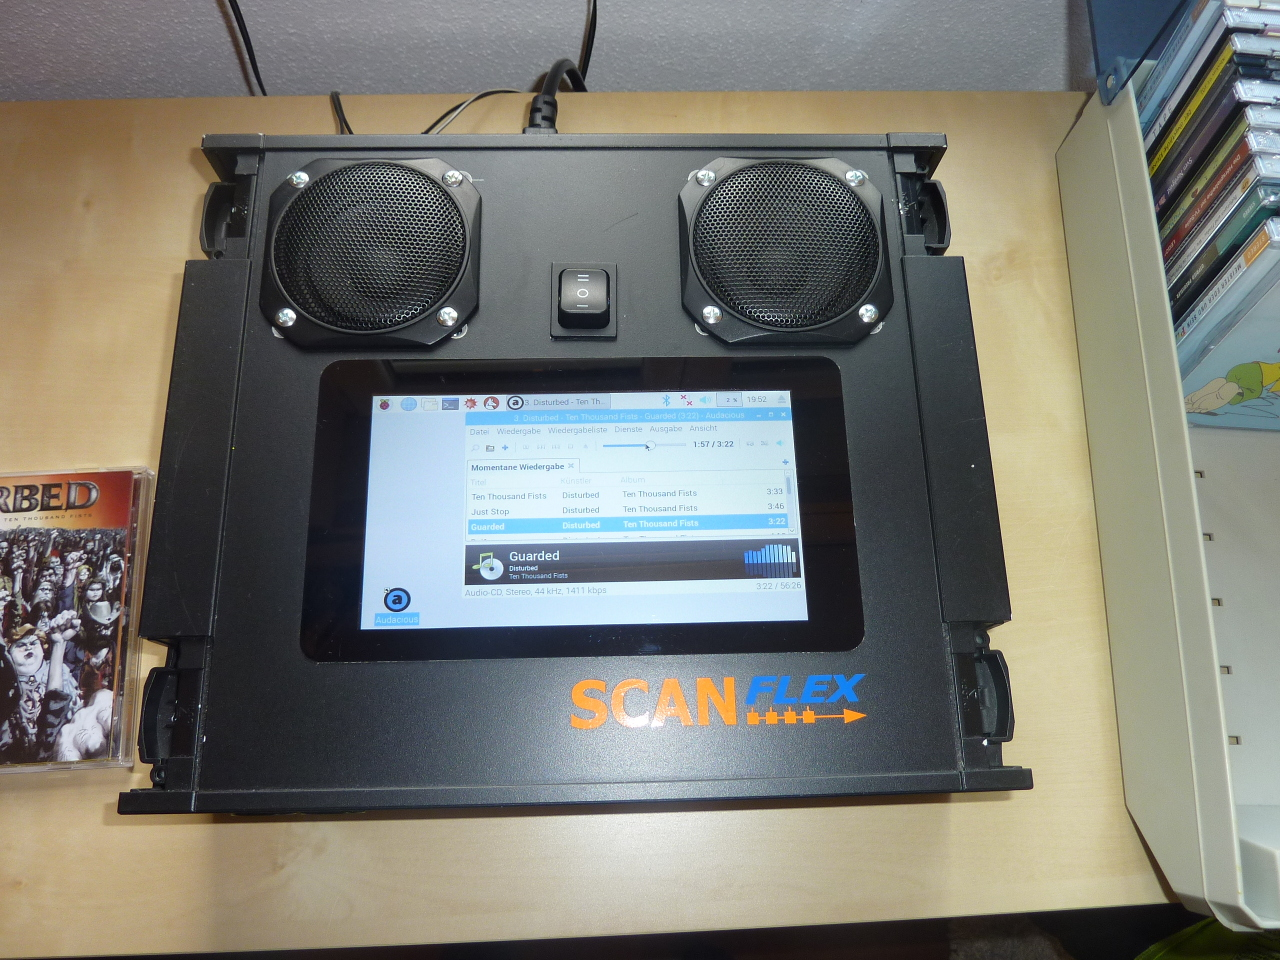
\includegraphics[width=12cm]{coverpic.jpg}
\end{figure}

%%------------------------------------------------------------------------------
%%   audacious icon, Copyright, CD player icon
%%------------------------------------------------------------------------------
\begin{tabular}{lllr}\\
\hline
% line with icons and copyright
\parbox[c][50px]{0.10\textwidth}{
\includegraphics[height=35px]{audacious.png}} & 
\parbox[c]{0.55\textwidth}{Simplified 2-clause BSD License\\ \copyright\ 2001--2018 by Audacious developers and others} &
\parbox[c]{0.15\textwidth}{Datum:\\13.04.2018} &
\parbox[c][50px]{0.10\textwidth}{
\includegraphics[height=35px]{tux.png}}\\
\hline
\end{tabular}

\end{center}

~\\
% coversheet.tex -- de (German)
% Language specific file of ../coversheet.tex
%
% This file contains language-specific texts.
Das Linux-Maskottchen \textit{Tux} wurde von \textit{Larry Ewing} mit 
dem Bildbearbeitungsprogramm \textit{GIMP} erstellt.\\
\url{mailto:lewing@isc.tamu.edu}
 % language-specific text line

\end{titlepage}

%\include{layout/abstract}
\cfoot{- \pagemark ~-}

\tableofcontents   % table of contents
\listoffigures     % list of figures
\listoftables      % list of tables
\renewcommand{\lstlistlistingname}{Verzeichnis der Listings}
%\lstlistoflistings % list of source code listings

%% list of abbreviations -------------------------------------------------------
%\input{Kapitel/Glossar}
%% for correct caption in the header line
%\clearpage\markboth{\nomname}{\nomname} 
%\printnomenclature
%\label{sec:Glossar}


% arabic page numbers in the main part -----------------------------------------
%%%%\clearpage
%%%%\pagenumbering{arabic}


% ##############################################################################
% ----------   including of chapters   -----------------------------------------
% ##############################################################################
% chapter1.tex -- de (German)
\chapter{Einleitung}

Vielen Dank f�r Ihr Interesse an {\autor}s {\Bezeichnung}.\\
Neben einem CD-Spieler befassen Sie sich hiermit gleichzeitig mit einem 
vollst�ndigen Computer auf Basis des {\RPi}, der Ihnen als Bastler viele 
weitere M�glichkeiten bietet. Lesen Sie diese Bedienungsanleitung durch, um 
das Ger�t vollst�ndig kennenzulernen und m�glicherweise sogar nachzubauen.

\section{Rechtliche Hinweise}
Bei der Konzeption des {\Bezeichnung}s wurde darauf geachtet, nur Software zu
verwenden, die unter einer freien Lizenz wie FreeBSD, GNU GPL oder �hnlichem zur
Verf�gung gestellt wird. 

\subsection*{Marken}
Einige Bezeichnungen in dieser Schrift k�nnen Marken sein, deren Benutzung durch
Dritte f�r deren Zwecke die Rechte der Inhaber verletzen k�nnen.

\subsection*{Links}
In dieser Bedienungsanleitung sind Links zu externen Seiten im Internet 
enthalten. Diese Inhalte macht sich der Verfasser {\autor} trotz Verlinkung
nicht zu eigen, da sie nicht in seinem Einflussbereich stehen! Zum Zeitpunkt der
Verlinkung waren keine rechtswidrigen Inhalte erkennnbar. Eine st�ndige 
�berpr�fung auf etwaige rechtsversto�ende �nderungen ist dem Verfasser nach
geltendem Recht nicht zuzumuten.\\
Sollten aktuelle oder k�nftige Inhalte jedoch rechtswidrig sein, so kann der
Autor dar�ber per e-mail an \url{mailto:schlizbaeda@gmx.de} informiert werden. 
Es werden dann entsprechende Ma�nahmen zur Beseitigung des/der betroffenen Links 
ergriffen.

\subsection*{DRM}
Die offizielle Lesart der Erfinder dieses Unfugs lautet \textit{Digital Rights
Management}, aber insbesondere die Freie-Software-Bewegung bezeichnet die unter
diesen Bereich fallenden technischen Verfahren treffender als \textit{Digital 
Restriction Management}, da viele dieser Verfahren mit den meisten 
Open-Source-Lizen\-zen nicht vereinbar sind.\\
Dies bedeutet jedoch \textbf{nicht}, dass DRM ignoriert werden darf! Vielmehr
wurde um 2003 dem Endverbraucher(!) in Deutschland durch die damalige Regierung
auferlegt, technisch nicht funktionierendes DRM (\zB einen Kopierschutz auf nicht
der Spezifikation entsprechenden Audio-CDs, sogenannten Un-CDs) selbst�ndig zu 
erkennen und entsprechende Ma�nahmen zur Einhaltung von DRM zu ergreifen. In den 
�brigen EU-Staaten d�rften �hnliche Gesetze existieren.\\
\textbf{F�r den {\Bezeichnung} kann nicht ausgeschlossen werden, dass einige
DRM-Ver\-fah\-ren technisch nicht erkannt und daher nicht automatisch 
ber�cksichtigt werden!}
Dies betrifft insbesondere mit einem sogenannten Kopierschutz versehene und
auf der H�lle durch ein entsprechendes Logo gekennzeichnete Un-CDs,
deren Inhalt streng genommen nicht einmal f�r die private Verwendung kopiert 
werden darf! Im wirklich pers�nlichen Umfeld werden derartige Verst��e derzeit 
in der Regel jedoch nicht polizeilich verfolgt\dots\\
\url{https://de.wikipedia.org/wiki/Digital_Rights_Management}

\subsection*{FreeBSD-Lizenz des Audioplayers {\audacious}\\{\audaciousStable}}
Copyright 2001-2017 Audacious developers and others

Redistribution and use in source and binary forms, with or without modification,
are permitted provided that the following conditions are met:

1. Redistributions of source code must retain the above copyright notice,
   this list of conditions, and the following disclaimer.

2. Redistributions in binary form must reproduce the above copyright notice,
   this list of conditions, and the following disclaimer in the documentation
   provided with the distribution.

This software is provided "{as} is"{ and} without any warranty, express or 
implied. In no event shall the authors be liable for any damages arising from 
the use of this software.

\url{https://audacious-media-player.org/download}

Im Rahmen dieser Lizenz wurde der Quellcode von {\audacious} mit dem Stand 
{\audaciousStable} von {\autor} f�r die Verwendung auf dem {\RPi} angepasst. Das 
Programm wurde um eine "`eject"'-Funktionalit�t erweitert, da das Bet�tigen der 
Auswurftaste des {CDROM}-Laufwerks bisweilen zu Aufh�ngern f�hrt. Weitere 
Informationen werden in Kapitel \ref{sect:compile} beschrieben.\\
Der Quellcode der ge�nderten Software kann �ber den folgenden Link 
heruntergeladen werden:\\
\url{https://github.com/schlizbaeda/audacious-raspiblaster}

\subsection*{Bildrechte}
Alle inhaltlich relevanten Fotos und technischen Abbildungen in diesem Dokument 
stammen vom Verfasser {\autor} selbst und werden hiermit von ihm unter der 
\textit{Creative-Commons}-Li\-zenz \textbf{CC-BY-SA 3.0} ver�ffentlicht. Sie 
d�rfen daher von jedem bei Namensnennung des Urhebers in unver�nderter oder 
auch in ver�nderter Form unter den gleichen Bedingungen weitergegeben werden:\\

\includegraphics[height=35px]{CC-BY-SA.png}

In dieser Bedienungsanleitung werden jedoch auch einige Icongrafiken aus 
anderen Quellen verwendet, die unter folgenden Lizenzen stehen:
\begin{table}[!h]
\centering
\renewcommand{\arraystretch}{2}
\begin{tabular}{|l|p{13.0cm}|}
\hline
                                                                    & Der Urheber \textit{Larry Ewing} gab die Grafik unter folgender Bedingung frei:\\
\parbox[c]{1.2cm}{~\newline 
\includegraphics[height=35px]{tux.png}} & "`Es ist erlaubt, diese Grafik zu verwenden und/oder zu ver�ndern.\newline
                                                                        Bedingung ist jedoch: Falls jemand fragt, muss man mich\newline
                                                                        -- lewing@isc.tamu.edu -- als Urheber nennen und auf GIMP hinweisen."'\\
\hline
\parbox[c]{1.2cm}{~\newline 
\includegraphics[height=35px]{rpiIcon.png}} & Himbeerlogo der {\foundation}:\newline \smaller{\url{https://static.raspberrypi.org/files/Raspberry_Pi_Visual_Guidelines_2018.pdf}}\\
\hline
\parbox[c]{1.2cm}{~\newline 
\includegraphics[height=35px]{audacious.png}} & Desktopicon des Audioplayers {\audacious}:\newline vermutlich CC-BY-SA?\\
\hline
\parbox[c]{1.2cm}{~\newline 
\includegraphics[height=35px]{raspiblaster.png}} & alternatives Desktopicon f�r einen Audioplayer auf dem {\Bezeichnung}:\newline CC-BY-SA U.S. (Autor: Wallpaper FX, \url{http://www.wallpaperfx.com/})\\
\hline
\end{tabular}
\vspace{0.5cm}
\caption{Lizensierung der Abbildungen}
\end{table}


\newpage
\section{Danksagung}
{\autor} m�chte folgenden Personen aus dem deutschen Raspberry Pi Forum\\ 
(\url{https://forum-raspberrypi.de}) seinen Dank aussprechen:

\textbf{@hyle} \url{https://forum-raspberrypi.de/user/36638-hyle/}:\\
Dieser Benutzer lieferte viele wertvolle Hinweise zum {\Bezeichnung}, 
insbesondere die Grund\-idee, die Auswurftaste des {\CDROM}-Laufwerks zu 
sperren.

\textbf{@smutbert} \url{https://forum-raspberrypi.de/user/21740-smutbert/}:\\
Eine echte Koryph�e um das Thema ALSA und dessen Konfigurarion und Einrichtung.

\textbf{@rpi444} \url{https://forum-raspberrypi.de/user/8097-rpi444/},\\
\textbf{@Tell} \url{https://forum-raspberrypi.de/user/9272-tell/}:\\
Die beiden zeigten den richtigen Weg auf, wie man es anpackt,
gro�e fremde C-/C++-Projekte erfolgreich zu kompilieren (Kapitel 
\ref{sect:compile}).


\newpage
\section{Konventionen dieser Bedienungsanleitung}
Folgende gestalterische Konventionen werden f�r diese Bedienungsanleitung 
festgelegt:

\begin{table}[!h]
\centering
\renewcommand{\arraystretch}{2}
\begin{tabular}{|p{3.5cm}|p{10.5cm}|}
\hline
\parbox[c]{3.5cm}{\begin{bclogo}[arrondi = 0.2, logo = \bcdanger, ombre = true, epOmbre = 0.25, couleurOmbre = red!75,blur]{Gefahr!} 
Text
\end{bclogo}} & Ein Gefahrenhinweis, dessen Nichtbeachtung zu \textbf{Personensch�den} und Ger�tesch�den f�hren kann!\\
\hline

\parbox[c]{3.5cm}{\begin{bclogo}[arrondi = 0.2, logo = \bcinfo, ombre = true, epOmbre = 0.25, couleurOmbre = black!30,blur]{Achtung} 
Text
\end{bclogo}} & Ein Gefahrenhinweis, dessen Nichtbeachtung zu Ger�tesch�den f�hren kann!\\
\hline

\parbox[c]{1em}{\begin{bclogo}[logo = \bclampe, noborder = true]{Hinweis}
Text
\end{bclogo}} & Ein Hinweis mit zus�tzlicher Information bzw. relevanter Erl�uterung zu einer bestimmten Funktionalit�t\\
\hline

\button{Schaltfl�che} & Kennzeichnung von Schaltfl�chen von Software\\
\hline
\menuitem{Men�punkt} & Kennzeichnung von Men�punkten von Software\\
\hline
\cmdPi{RPi-Kommando} & bash-Kommando am {\RPi}\\
\hline
\cmdPC{PC-Kommando} & Kommandozeile am Linux-PC\\
\hline
\cmdWin{PC-Kommando} & alternativ:\newline Kommandozeile am Windows-PC\\
\hline
\comment{Kommentar} & Kommentar in einer Kommandozeile\\
\hline
\stdout{Meldung} & Kennzeichnung von Meldungen der Software \textbf{\Bezeichnung}\\
\hline
\end{tabular}
\vspace{0.5cm}
\caption{Konventionen der Dokumentation}
\end{table}


%\parbox[c]{\textwidth}{\begin{bclogo}[arrondi = 0.2, logo = \bcdanger, ombre = true, epOmbre = 0.25, couleurOmbre = black!30,blur]{Gefahr} 
%Dieses Symbol warnt vor gef�hrlichen Spannungen  
%\end{bclogo}}	
%
%\parbox[c]{\textwidth}{\begin{bclogo}[arrondi = 0.2, logo = \bcdanger, ombre = true, epOmbre = 0.25, couleurOmbre = black!30,blur]{Gefahr} 
%Dieses Symbol warnt vor gef�hrlichen Spannungen  
%\end{bclogo}}	
%

%\parbox[c]{1em}{\begin{bclogo}[logo = \bclampe, noborder = true]{Hinweis} Text \end{bclogo}
%\parbox[c]{3.5cm}{\begin{bclogo}[arrondi = 0.2, logo = \bcattention, ombre = true, epOmbre = 0.25, couleurOmbre = black!30,blur]{logo} attention \end{bclogo}}	
%\parbox[c]{3.5cm}{\begin{bclogo}[arrondi = 0.2, logo = \bcbombe, ombre = true, epOmbre = 0.25, couleurOmbre = black!30,blur]{logo} bombe \end{bclogo}}	
%\parbox[c]{3.5cm}{\begin{bclogo}[arrondi = 0.2, logo = \bcbook, ombre = true, epOmbre = 0.25, couleurOmbre = black!30,blur]{logo} book \end{bclogo}}	
%\parbox[c]{3.5cm}{\begin{bclogo}[arrondi = 0.2, logo = \bccalendrier, ombre = true, epOmbre = 0.25, couleurOmbre = black!30,blur]{logo} calendrier \end{bclogo}}	
%\parbox[c]{3.5cm}{\begin{bclogo}[arrondi = 0.2, logo = \bcclefa, ombre = true, epOmbre = 0.25, couleurOmbre = black!30,blur]{logo} clefa \end{bclogo}}	
%\parbox[c]{3.5cm}{\begin{bclogo}[arrondi = 0.2, logo = \bccle, ombre = true, epOmbre = 0.25, couleurOmbre = black!30,blur]{logo} cle \end{bclogo}}	
%\parbox[c]{3.5cm}{\begin{bclogo}[arrondi = 0.2, logo = \bcclesol, ombre = true, epOmbre = 0.25, couleurOmbre = black!30,blur]{logo} clesol \end{bclogo}}	
%\parbox[c]{3.5cm}{\begin{bclogo}[arrondi = 0.2, logo = \bccoeur, ombre = true, epOmbre = 0.25, couleurOmbre = black!30,blur]{logo} coeur \end{bclogo}}	
%\parbox[c]{3.5cm}{\begin{bclogo}[arrondi = 0.2, logo = \bccrayon, ombre = true, epOmbre = 0.25, couleurOmbre = black!30,blur]{logo} crayon \end{bclogo}}	
%\parbox[c]{3.5cm}{\begin{bclogo}[arrondi = 0.2, logo = \bccube, ombre = true, epOmbre = 0.25, couleurOmbre = black!30,blur]{logo} cube \end{bclogo}}	
%\parbox[c]{3.5cm}{\begin{bclogo}[arrondi = 0.2, logo = \bcdanger, ombre = true, epOmbre = 0.25, couleurOmbre = black!30,blur]{logo} danger \end{bclogo}}	
%\parbox[c]{3.5cm}{\begin{bclogo}[arrondi = 0.2, logo = \bcdallemagne, ombre = true, epOmbre = 0.25, couleurOmbre = black!30,blur]{logo} dallemagne \end{bclogo}}	
%\parbox[c]{3.5cm}{\begin{bclogo}[arrondi = 0.2, logo = \bcdautriche, ombre = true, epOmbre = 0.25, couleurOmbre = black!30,blur]{logo} dautriche \end{bclogo}}	
%\parbox[c]{3.5cm}{\begin{bclogo}[arrondi = 0.2, logo = \bcdbelgique, ombre = true, epOmbre = 0.25, couleurOmbre = black!30,blur]{logo} dbelgique \end{bclogo}}	
%\parbox[c]{3.5cm}{\begin{bclogo}[arrondi = 0.2, logo = \bcdbulgarie, ombre = true, epOmbre = 0.25, couleurOmbre = black!30,blur]{logo} dbulgarie \end{bclogo}}	
%\parbox[c]{3.5cm}{\begin{bclogo}[arrondi = 0.2, logo = \bcdfrance, ombre = true, epOmbre = 0.25, couleurOmbre = black!30,blur]{logo} dfrance \end{bclogo}}	
%\parbox[c]{3.5cm}{\begin{bclogo}[arrondi = 0.2, logo = \bcditalie, ombre = true, epOmbre = 0.25, couleurOmbre = black!30,blur]{logo} ditalie \end{bclogo}}	
%\parbox[c]{3.5cm}{\begin{bclogo}[arrondi = 0.2, logo = \bcdluxembourg, ombre = true, epOmbre = 0.25, couleurOmbre = black!30,blur]{logo} dluxembourg \end{bclogo}}	
%\parbox[c]{3.5cm}{\begin{bclogo}[arrondi = 0.2, logo = \bcdpaysbas, ombre = true, epOmbre = 0.25, couleurOmbre = black!30,blur]{logo} dpaysbas \end{bclogo}}	
%\parbox[c]{3.5cm}{\begin{bclogo}[arrondi = 0.2, logo = \bcdz, ombre = true, epOmbre = 0.25, couleurOmbre = black!30,blur]{logo} dz \end{bclogo}}	
%\parbox[c]{3.5cm}{\begin{bclogo}[arrondi = 0.2, logo = \bceclaircie, ombre = true, epOmbre = 0.25, couleurOmbre = black!30,blur]{logo} eclaircie \end{bclogo}}	
%\parbox[c]{3.5cm}{\begin{bclogo}[arrondi = 0.2, logo = \bcetoile, ombre = true, epOmbre = 0.25, couleurOmbre = black!30,blur]{logo} etoile \end{bclogo}}	
%\parbox[c]{3.5cm}{\begin{bclogo}[arrondi = 0.2, logo = \bcfemme, ombre = true, epOmbre = 0.25, couleurOmbre = black!30,blur]{logo} femme \end{bclogo}}	
%\parbox[c]{3.5cm}{\begin{bclogo}[arrondi = 0.2, logo = \bcfeujaune, ombre = true, epOmbre = 0.25, couleurOmbre = black!30,blur]{logo} feujaune \end{bclogo}}	
%\parbox[c]{3.5cm}{\begin{bclogo}[arrondi = 0.2, logo = \bcfeurouge, ombre = true, epOmbre = 0.25, couleurOmbre = black!30,blur]{logo} feurouge \end{bclogo}}	
%\parbox[c]{3.5cm}{\begin{bclogo}[arrondi = 0.2, logo = \bcfeutricolore, ombre = true, epOmbre = 0.25, couleurOmbre = black!30,blur]{logo} feutricolore \end{bclogo}}	
%\parbox[c]{3.5cm}{\begin{bclogo}[arrondi = 0.2, logo = \bcfeuvert, ombre = true, epOmbre = 0.25, couleurOmbre = black!30,blur]{logo} feuvert \end{bclogo}}	
%\parbox[c]{3.5cm}{\begin{bclogo}[arrondi = 0.2, logo = \bcfleur, ombre = true, epOmbre = 0.25, couleurOmbre = black!30,blur]{logo} fleur \end{bclogo}}	
%\parbox[c]{3.5cm}{\begin{bclogo}[arrondi = 0.2, logo = \bchomme, ombre = true, epOmbre = 0.25, couleurOmbre = black!30,blur]{logo} homme \end{bclogo}}	
%\parbox[c]{3.5cm}{\begin{bclogo}[arrondi = 0.2, logo = \bchorloge, ombre = true, epOmbre = 0.25, couleurOmbre = black!30,blur]{logo} horloge \end{bclogo}}	
%\parbox[c]{3.5cm}{\begin{bclogo}[arrondi = 0.2, logo = \bcicosaedre, ombre = true, epOmbre = 0.25, couleurOmbre = black!30,blur]{logo} icosaedre \end{bclogo}}	
%\parbox[c]{3.5cm}{\begin{bclogo}[arrondi = 0.2, logo = \bcinfo, ombre = true, epOmbre = 0.25, couleurOmbre = black!30,blur]{logo} info \end{bclogo}}	
%\parbox[c]{3.5cm}{\begin{bclogo}[arrondi = 0.2, logo = \bcinterdit, ombre = true, epOmbre = 0.25, couleurOmbre = black!30,blur]{logo} interdit \end{bclogo}}	
%\parbox[c]{3.5cm}{\begin{bclogo}[arrondi = 0.2, logo = \bclampe, ombre = true, epOmbre = 0.25, couleurOmbre = black!30,blur]{logo} lampe \end{bclogo}}	
%\parbox[c]{3.5cm}{\begin{bclogo}[arrondi = 0.2, logo = \bcloupe, ombre = true, epOmbre = 0.25, couleurOmbre = black!30,blur]{logo} loupe \end{bclogo}}	
%\parbox[c]{3.5cm}{\begin{bclogo}[arrondi = 0.2, logo = \bcneige, ombre = true, epOmbre = 0.25, couleurOmbre = black!30,blur]{logo} neige \end{bclogo}}	
%\parbox[c]{3.5cm}{\begin{bclogo}[arrondi = 0.2, logo = \bcnote, ombre = true, epOmbre = 0.25, couleurOmbre = black!30,blur]{logo} note \end{bclogo}}	
%\parbox[c]{3.5cm}{\begin{bclogo}[arrondi = 0.2, logo = \bcnucleaire, ombre = true, epOmbre = 0.25, couleurOmbre = black!30,blur]{logo} nucleaire \end{bclogo}}	
%\parbox[c]{3.5cm}{\begin{bclogo}[arrondi = 0.2, logo = \bcoctaedre, ombre = true, epOmbre = 0.25, couleurOmbre = black!30,blur]{logo} octaedre \end{bclogo}}	
%\parbox[c]{3.5cm}{\begin{bclogo}[arrondi = 0.2, logo = \bcoeil, ombre = true, epOmbre = 0.25, couleurOmbre = black!30,blur]{logo} oeil \end{bclogo}}	
%\parbox[c]{3.5cm}{\begin{bclogo}[arrondi = 0.2, logo = \bcorne, ombre = true, epOmbre = 0.25, couleurOmbre = black!30,blur]{logo} orne \end{bclogo}}	
%\parbox[c]{3.5cm}{\begin{bclogo}[arrondi = 0.2, logo = \bcours, ombre = true, epOmbre = 0.25, couleurOmbre = black!30,blur]{logo} ours \end{bclogo}}	
%\parbox[c]{3.5cm}{\begin{bclogo}[arrondi = 0.2, logo = \bcoutil, ombre = true, epOmbre = 0.25, couleurOmbre = black!30,blur]{logo} outil \end{bclogo}}	
%\parbox[c]{3.5cm}{\begin{bclogo}[arrondi = 0.2, logo = \bcpeaceandlove, ombre = true, epOmbre = 0.25, couleurOmbre = black!30,blur]{logo} peaceandlove \end{bclogo}}	
%\parbox[c]{3.5cm}{\begin{bclogo}[arrondi = 0.2, logo = \bcpluie, ombre = true, epOmbre = 0.25, couleurOmbre = black!30,blur]{logo} pluie \end{bclogo}}	
%\parbox[c]{3.5cm}{\begin{bclogo}[arrondi = 0.2, logo = \bcplume, ombre = true, epOmbre = 0.25, couleurOmbre = black!30,blur]{logo} plume \end{bclogo}}	
%\parbox[c]{3.5cm}{\begin{bclogo}[arrondi = 0.2, logo = \bcpoisson, ombre = true, epOmbre = 0.25, couleurOmbre = black!30,blur]{logo} poisson \end{bclogo}}	
%\parbox[c]{3.5cm}{\begin{bclogo}[arrondi = 0.2, logo = \bcrecyclage, ombre = true, epOmbre = 0.25, couleurOmbre = black!30,blur]{logo} recyclage \end{bclogo}}	
%\parbox[c]{3.5cm}{\begin{bclogo}[arrondi = 0.2, logo = \bcrosevents, ombre = true, epOmbre = 0.25, couleurOmbre = black!30,blur]{logo} rosevents \end{bclogo}}	
%\parbox[c]{3.5cm}{\begin{bclogo}[arrondi = 0.2, logo = \bcsmiley-bonnehumeur, ombre = true, epOmbre = 0.25, couleurOmbre = black!30,blur]{logo} smiley-bonnehumeur \end{bclogo}}	
%\parbox[c]{3.5cm}{\begin{bclogo}[arrondi = 0.2, logo = \bcsmiley-mauvaisehumeur, ombre = true, epOmbre = 0.25, couleurOmbre = black!30,blur]{logo} smiley-mauvaisehumeur \end{bclogo}}	
%\parbox[c]{3.5cm}{\begin{bclogo}[arrondi = 0.2, logo = \bcsoleil, ombre = true, epOmbre = 0.25, couleurOmbre = black!30,blur]{logo} soleil \end{bclogo}}	
%\parbox[c]{3.5cm}{\begin{bclogo}[arrondi = 0.2, logo = \bcstop, ombre = true, epOmbre = 0.25, couleurOmbre = black!30,blur]{logo} stop \end{bclogo}}	
%\parbox[c]{3.5cm}{\begin{bclogo}[arrondi = 0.2, logo = \bctakecare, ombre = true, epOmbre = 0.25, couleurOmbre = black!30,blur]{logo} takecare \end{bclogo}}	
%\parbox[c]{3.5cm}{\begin{bclogo}[arrondi = 0.2, logo = \bctetraedre, ombre = true, epOmbre = 0.25, couleurOmbre = black!30,blur]{logo} tetraedre \end{bclogo}}	
%\parbox[c]{3.5cm}{\begin{bclogo}[arrondi = 0.2, logo = \bctrefle, ombre = true, epOmbre = 0.25, couleurOmbre = black!30,blur]{logo} trefle \end{bclogo}}	
%\parbox[c]{3.5cm}{\begin{bclogo}[arrondi = 0.2, logo = \bctrombone, ombre = true, epOmbre = 0.25, couleurOmbre = black!30,blur]{logo} trombone \end{bclogo}}	
%\parbox[c]{3.5cm}{\begin{bclogo}[arrondi = 0.2, logo = \bcvaletcoeur, ombre = true, epOmbre = 0.25, couleurOmbre = black!30,blur]{logo} valetcoeur \end{bclogo}}	
%\parbox[c]{3.5cm}{\begin{bclogo}[arrondi = 0.2, logo = \bcvelo, ombre = true, epOmbre = 0.25, couleurOmbre = black!30,blur]{logo} velo \end{bclogo}}	
%\parbox[c]{3.5cm}{\begin{bclogo}[arrondi = 0.2, logo = \bcyin, ombre = true, epOmbre = 0.25, couleurOmbre = black!30,blur]{logo} yin \end{bclogo}}	
%

%% Diese Auflistung k�nnte irgendwann notwendig werden,
%% wenn auf Github verschiedene Versionsst�nde herumgeistern und die
%% einzelnen Nutzer evtl. verschiedene St�nde vorliegen haben...
%Ausgabest�nde dieser Dokumentation:
%
%\begin{tabular}{llp{0.70\textwidth}}
%\textbf{Version 1} & 20.02.2016 & Erstversion f�r Programmversion V0.1\\
%\textbf{Version 2} & 01.07.2016 & zus�tzliche Hinweise zur Software-Installation von Version V0.1\\
%\textbf{Version 3} & 18.08.2017 & {\Bezeichnung} {\Version}\\
%\end{tabular}


\section{Kurzbeschreibung}
Der {\Bezeichnung} ist ein CD-Spieler mit eingebautem Stereoverst�rker 
(\hardware{HifiBerry MiniAMP}) und Lautsprechern, mit einer (zumindest in 
technischer Hinsicht) entfernten �hnlichkeit zu den seit den 80er-Jahren 
bekannten Ger�ten, die im Volksmund auch als \textit{Ghettoblaster} bezeichnet 
werden. Er besteht aus einem {\RPi} 3B, an dem intern �ber einen seiner 
USB-An\-schl�s\-se ein handels�bliches \CDROM-Laufwerk (\hardware{LG \LGdrive}, 
eigentlich ein DVD-Brenner) angeschlossen ist. Die Bedienung des {\Bezeichnung}s 
erfolgt �ber das von der {\foundation} herausgebrachte 7-Zoll {\raspidisplay}.\\
Neben den internen Lautsprechern k�nnen an der R�ckseite auch externe 
Lautsprecherboxen angeschlossen werden. Zwei weitere USB-Anschl�sse und die
Ethernetbuchse des {\RPi} sind �ber Neutrikstecker von au�en zug�nglich.\\
Die Spannungsversorgung erfolgt �ber das 230V-Stromnetz. Im {\Bezeichnung} ist 
daf�r ein Einbaunetzteil (\hardware{Meanwell RS-25-05}: 5V, 5A) verbaut, das alle 
Komponenten mit ausreichenden Leistungsreserven versorgt.

Softwareseitig erfolgt auf dem {\Bezeichnung} die Wiedergabe von Audio-CDs �ber 
das Open-Source-Programm {\audacious}, das derzeit als {\audaciousStable} 
vorliegt. 

\subsection*{Ausblick auf geplante Erweiterungen}
\begin{compactitem}
\item{Batteriebetrieb}
\item{Hardwaretaster und/oder Drehgeber �ber GPIOs f�r Lautst�rke etc.}
\item{Mediaplayer f�r USB-Sticks}
\item{CD rippen mit \texttt{abcde}}
\item{DVD-Betrieb (mit kodi-Betriebssystem)}
\item{Bluetooth-"`Lautsprecher"'}
\item{UKW- und/oder DAB+-Betrieb}
\end{compactitem}


\section{St�ckliste}
\begin{table}[!h]
\centering
\renewcommand{\arraystretch}{1.25}
\begin{tabular}{|r|l|p{2.6cm}|p{5.0cm}|l|p{2.7cm}|}
\hline
\textbf{x}	&	\textbf{Hersteller}	&	\textbf{Typ}	&	\textbf{Bezeichnung}			&	\textbf{Lieferant}	&	\textbf{Bestellnr.}\\
\hline
		1		&	bopla				&	68626120		&	Botego BO 62612\newline
																Geh�use geschlossen\newline
																308mm x 257mm x 81mm			&	?					&	Altbestand\\
		1		&	Schurter			&	6762			&	Ger�teeinbaustecker-Kombination	&	B�rklin				&	41 F 139\\
		2		&	RND					&	170-00020		&	Feinsicherung tr�ge 1A			&	reichelt			&	RND 170-00020\\
		1		&	MeanWell			&	RS 25-5			&	Schaltnetzteil 25W, 5V, 5A		&	reichelt			&	SNT RS 25 5\\
	%	1		&	{\foundation}		&	?				&	{\raspidisplay}					&	www.raspiprojekt.de	&	TS7DSI\\
	%	1		&	{\foundation}		&	RPi 3B			&	Raspberry Pi 3B					&	www.raspiprojekt.de	&	RASPI3B\\
		1		&	Foundation			&	-				&	{\raspidisplay}					&	raspiprojekt		&	TS7DSI\\
		1		&	Foundation			&	RPi 3B			&	Raspberry Pi 3B					&	raspiprojekt		&	RASPI3B\\
\hline
\end{tabular}
\vspace{0.5cm}
\caption{St�ckliste -- Teil 1}
\end{table}

\begin{table}[!h]
\centering
\renewcommand{\arraystretch}{1.25}
\begin{tabular}{|r|l|p{2.6cm}|p{5.0cm}|l|p{2.7cm}|}
\hline
\textbf{x}	&	\textbf{Hersteller}	&	\textbf{Typ}	&	\textbf{Bezeichnung}			&	\textbf{Lieferant}	&	\textbf{Bestellnr.}\\
\hline
		1		&	HifiBerry			&	MiniAMP	V1.0	&	Stereoverst�rker\newline
																2x3W Musikleistung				&	reichelt			&	RPI HB\newline MINI AMP\\
		2		&	Visaton				&	SC 8 N 8Ohm		&	Lautsprecher 30W, 8Ohm			&	reichelt			&	VIS SC 8N-8\\
	%	2		&	Visaton				& 	GRILLE FRS 8	&	Lautsprecherabdeckung\newline
	%															82mm x 82mm						&	RS Components GmbH	&	4538953\\
		2		&	Visaton				& 	GRILLE FRS 8	&	Lautsprecherabdeckung\newline
																82mm x 82mm						&	RS 					&	4538953\\
	%	1		&	?					&					&	Lautsprecheranschluss 4-fach	&	RS Components GmbH	&	392683\\
	%	1       &	Marquardt			&	1839.0105		&	Wippschalter 2P I/O/II\newline
	%															30mm x 22mm schwarz				&	RS Components GmbH	&	7410823\\
		1		&	?					&					&	Lautsprecheranschluss 4-fach	&	RS 				 	&	392683\\
		1       &	Marquardt			&	1839.0105		&	Wippschalter 2P I/O/II\newline
																30mm x 22mm schwarz				&	RS 				 	&	7410823\\

		1		&	LG					&	\LGdrive		&	Slim Line DVD-Writer			&	Laden				&	vor Ort\\
		2		&	Neutrik				&	NAUSB-W-B		&	USB-Einbaubuchse				&	reichelt			&	NAUSB-WB\\
		1		&	Neutrik				&	NE8FDX-P6		&	Ethernetbuchse Cat.6A			& 	reichelt			&	CAT6A BU BK\\
		1		&	schlizb�da			&	Eigenbau		&	Relaisansteuerung f�r GPIO4		&						&	\\
\hline
\end{tabular}
\vspace{0.5cm}
\caption{St�ckliste - Teil 2}
\end{table}

Die diversen Kleinteile wie Schrauben, Verbindungskabel (Ethernet, USB, Eigenbau)
sind in dieser St�ckliste nicht einzeln aufgef�hrt.


\section{Technische Daten}
\renewcommand{\arraystretch}{1.25}

\subsection{Spannungsversorgung}
\begin{tabular}{p{5.0cm}p{10.0cm}}
Netzspannung				&	88VAC -- 264VAC\\
Netzfrequenz				&	47Hz -- 63Hz\\
Stromaufnahme bei 230VAC	&	0,4A\\
Sekund�rspannung			&	5V\\
Sekund�rstrom				&	5A\\
Sekund�rleistung			&	25W\\
\end{tabular}

\subsection{Audioverst�rker (HifiBerry MiniAMP)}
\begin{tabular}{p{5.0cm}p{10.0cm}}
Verst�rkertyp				&	HifiBerry MiniAMP V1.0 (Class-D Verst�rker)\\
Musikleistung				&	2 x 3W (max.)\\
Samplerate					&	44,1kHz -- 192kHz\\
\end{tabular}

\subsection{\RPi}
\begin{tabular}{p{5.0cm}p{10.0cm}}
{\RPi} Version				&	{\RPi} 3B\\
SoC (Broadcom)				&	BCM2837\\
Architektur					&	ARM Cortex-A53 (quad core)\\
Taktrate CPU				&	1200MHz\\
Taktrate GPU				&	300MHz/400MHz\\
Arbeitsspeicher				&	1GB\\
Nichtfl�chtiger Speicher	&	abh�ngig von der verwendeten SD-Karte\newline
								mind. 8GB f�r Raspbian Stretch Desktop erforderlich\\
\end{tabular}
\textbf{Verwendete GPIOs}\\
\begin{tabular}{p{5.0cm}p{10.0cm}}
GPIO 4						&	Pin \textbf{7}: Relaisansteuerung f�r die eject-Sperre\\
GPIO 2, 3					&   Pins \textbf{3}, \textbf{5}: MiniAMP I2C-Bus\\
GPIO 18 -- 21				&   Pins \textbf{12}, \textbf{35}, \textbf{38}, \textbf{40}: MiniAMP I2S-Bus\\
GPIO 26						&	Pin \textbf{37}: MiniAmp shut down power stage\\
ID SDA, ID SCL				&	Pins \textbf{27}, \textbf{28}: I2C-EEPROM mit Ger�tedaten
\end{tabular}

\subsection{Laufwerk (LG \LGdrive)}
\begin{tabular}{p{5.0cm}p{10.0cm}}
Unterst�tzte Disk-Formate	&	\mbox{DVD-ROM} (Single/Dual), \mbox{DVD-RW}, 
								\mbox{DVD-R}, \mbox{DVD+RW}, \mbox{DVD+R}, 
								\mbox{DVD+R} Double layer, \mbox{DVD-R} Dual 
								layer, \mbox{DVD-RAM}, \mbox{M-Disc} 
								\mbox{(DVD+R SL)}, \mbox{CDDA} (CD Digital Audio)
								\& \mbox{CD-Extra}, \mbox{CD-Plus}, 
								\mbox{CD-ROM}, \mbox{CD-ROM XA-Ready}, 
								\mbox{CD-I FMV}, \mbox{CD-TEXT}, 
								\mbox{CD-Bridge}, \mbox{CD-R}, \mbox{CD-RW},
								\mbox{Photo-CD} (Single- \& Multi-Session),
								\mbox{Video CD}, \mbox{DVD-VIDEO}\\
\end{tabular}
\begin{tabular}{p{5.0cm}p{10.0cm}}
Lesegeschwindigkeiten		&	DVD-R/RW/ROM: 8x/8x/8x max.\newline
								DVD-R DL: 8x max.\newline
								DVD-RAM (Ver.2.2 \& Higher): 6x max.\newline
								M-Disc (DVD+R SL): 8x max.\newline
								DVD-Video (CSS Compliant Disc) : 4x max.\newline
								DVD+R/+RW: 8x/8x max.\newline
								DVD+R DL: 8x max.\newline
								CD-R/RW/ROM: 24x/24x/24x max.\newline
								CD-DA (DAE): 24x max.\\
\end{tabular}
\begin{tabular}{p{5.0cm}p{10.0cm}}
Schreibgeschwindigkeiten	&	DVD-R: 2x, 4x, 8x\newline
								DVD-R DL: 2x, 4x, 6x\newline
								DVD-RW: 2x, 4x, 6x\newline
								DVD-RAM (Ver. 2.2 \& higher): 2x, 3x, 5x\newline
								M-Disc (DVD+R SL): 4x\newline
								DVD+R: 2.4x, 4x, 8x\newline
								DVD+R DL: 2.4x, 4x, 6x\newline
								DVD+RW: 2.4x, 3.3x, 4x, 8x\newline
								CD-R: 10x, 16x, 24x\newline
								CD-RW: 4x, 10x, 16x, 24x\\
\end{tabular}
\begin{tabular}{p{5.0cm}p{10.0cm}}
Anschluss					&	USB 2.0\\
Spannungsversorgung			&	5V DC\\
max. Stromaufnahme			&	1,6A\\
\end{tabular}

\textbf{Daten�bertragungsrate}\\		
\begin{tabular}{p{5.0cm}p{10.0cm}}
Sustained					&	CD-ROM: 3,600 kB/s (24x max)\newline
								DVD-ROM: 11.08 MB/s (8x max)\newline
								CD-ROM: 140 ms (typisch)\newline
								DVD-ROM: 160 ms (typisch)\newline
								DVD-RAM: 200 ms (typisch)\\
Buffer capacity				&	0.75 MB\\
MTBF						&	60000 Stunden "`Power On"' (Duty Cycle 10\%)\\
\end{tabular}

\textbf{Umgebungsbedingungen (Betrieb)}\\
\begin{tabular}{p{5.0cm}p{10.0cm}}
Temperatur					&	5�C to 40�C\\
rel. Luftfeuchtigkeit		&	15\% bis 85\%\\
\end{tabular}

\textbf{Umgebungsbedingungen (Lagerung)}\\
\begin{tabular}{p{5.0cm}p{10.0cm}}
Temperatur					&	-30�C to 60�C\\
rel. Luftfeuchtigkeit		&	10\% to 90\%\\
\end{tabular}

% chapter2.tex -- de (German)
\chapter{Bedienungsanleitung}

Dieses Kapitel ist eine klassische Bedienungsanleitung f�r Benutzer, die den
{\Bezeichnung} normal verwenden, ohne dabei die Software oder Hardware des 
Ger�tes zu ver�ndern.


\section{Einschalten}
Zum Einschalten des {\Bezeichnung}s muss der Hauptschalter auf der R�ckseite des 
Ger�tes in Stellung I geschaltet werden. Es wird der Bootvorgang des {\RPi} 
gestartet und das Betriebssystem auf der SD-Karte (Raspbian Stretch Desktop vom
13.03.2018) wird in den Arbeitsspeicher geladen. Nach ca. 10 Sekunden ist der 
Bootvorgang abgeschlossen und auf dem Display erscheint der Desktop (siehe 
Abbildung \ref{fig:desktop00}).

\begin{figure}[h]
\centering
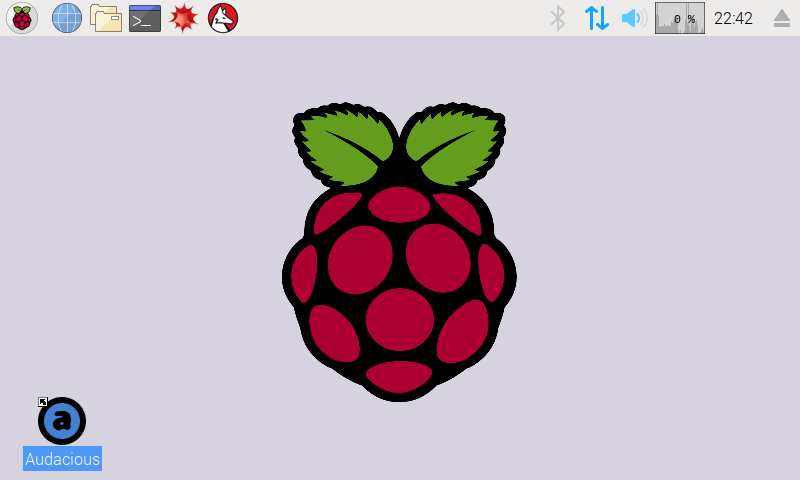
\includegraphics[width=0.8\textwidth]{desktop00.png}
\caption{Raspbian Stretch Desktop}
\label{fig:desktop00}
\end{figure}


\section{{\Bezeichnung} herunterfahren und ausschalten}
Wie jeder Computer muss auch der {\Bezeichnung} sauber beendet werden!  
Zun�chst muss das Betriebssystem (Raspbian Stretch Desktop) �ber den Men�punkt 
\menuitem{\rpiIcon$\rightarrow$Shutdown...$\rightarrow$He\-runterfahren}
heruntergefahren werden. Nachdem das Display schwarz geworden ist, muss nochmals 
f�r ca. 10 Sekunden gewartet werden, bevor der Strom �ber den Hauptschalter auf 
der Ger�ter�ckseite abgeschaltet werden darf.

\begin{figure}[h]
\centering
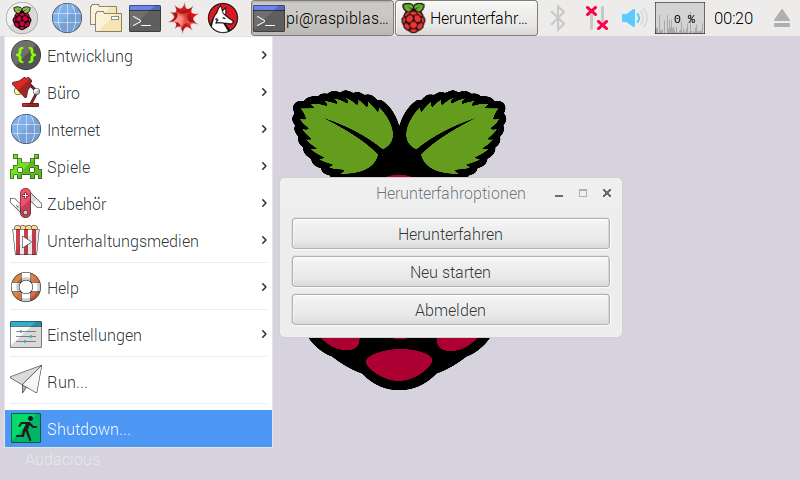
\includegraphics[width=0.8\textwidth]{\lang/desktop08.png}
\caption{{\Bezeichnung} herunterfahren}
\label{fig:desktop08}
\end{figure}

\begin{bclogo}[arrondi = 0.2, logo = \bcinfo, ombre = true, epOmbre = 0.25, couleurOmbre = black!30,blur]{Achtung}
Vor dem Abschalten der Stromversorgung ist daf�r zu sorgen, dass der {\RPi} 
vorher \textbf{komplett} heruntergefahren ist! Bei unkontrolliertem Ausschalten 
kann es ansonsten vorkommen, dass der Strom \textit{genau w�hrend eines 
Schreibzugriffes auf die SD-Karte} weggenommen wird. Dieser dadurch 
m�glicherweise unvollst�ndige oder fehlerhafte Schreibzugriff kann das 
Dateisystem auf der SD-Karte auf undefinierte Weise besch�digen. Auch wenn dies
zu 99\% der F�lle nicht eintritt, so sollte es dennoch vermieden werden, um 
einem Datenverlust auf der SD-Karte vorzubeugen! 
\end{bclogo}


\section{Lautst�rke einstellen}
In der Taskleiste von Raspbian befindet sich rechts oben ein Laustprechersymbol.
Durch Klick auf dieses Symbol wird ein grafisches Steuerelement in Form eines 
Schiebereglers ge�ffnet, mit dem die Wiedergabelautst�rke eingestellt werden 
kann. Die Anzahl der angedeuteten Schallwellen (1 -- 3) zeigt grob die 
eingestellte Lautst�rke an. Ein rotes \textcolor{red}{\texttt{x}} bedeutet
dabei die Stummschaltung der Audiowiedergabe.


\section{Starten des Audioplayers \audacious}
Die CD-Wiedergabe erfolgt �ber das Programm {\audacious} -- {\audaciousStable}. 
Diese Software kann entweder �ber den Men�punkt 
\menuitem{\rpiIcon$\rightarrow$Unterhaltungsme\-dien$\rightarrow$Audacious} 
gestartet werden oder durch einen Doppelklick auf das Icon "`Audacious"' in der 
linken unteren Ecke des Desktops.


\section{CD einlegen und Wiedergabe starten}
Zun�chst wird das Laufwerk �ber die Auswurftaste ge�ffnet und die gew�nschte CD 
eingelegt (siehe Abbildung \ref{fig:insertCD}) und das Laufwerk wieder 
geschlossen.

\begin{figure}[h]
\centering
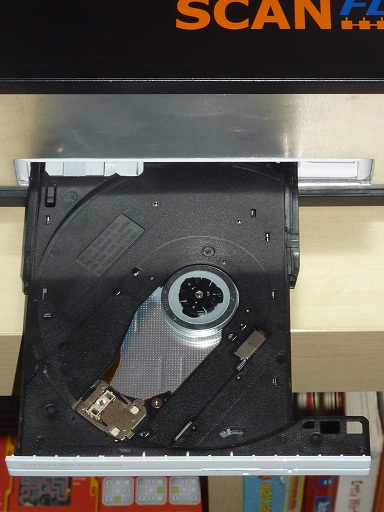
\includegraphics[width=0.4\textwidth]{tray_empty.jpg}
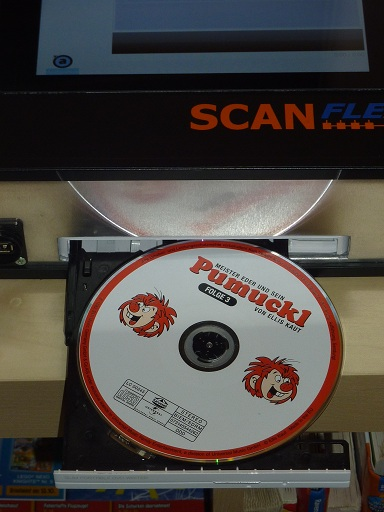
\includegraphics[width=0.4\textwidth]{tray_CD.jpg}
\caption{CD in Laufwerksschublade einlegen}
\label{fig:insertCD}
\end{figure}

Nach kurzer Zeit hat das Laufwerk die CD vollst�ndig eingelesen und Raspbian
�ffnet das Betriebssystemfenster \dialogbox{Wechseldatentr�ger wurde eingelegt}. 
Jetzt ist die CD zum Abspielen bereit und dieses Fenster kann mit der 
Schaltfl�che \button{Abbrechen} geschlossen werden. 

\begin{figure}[h]
\centering
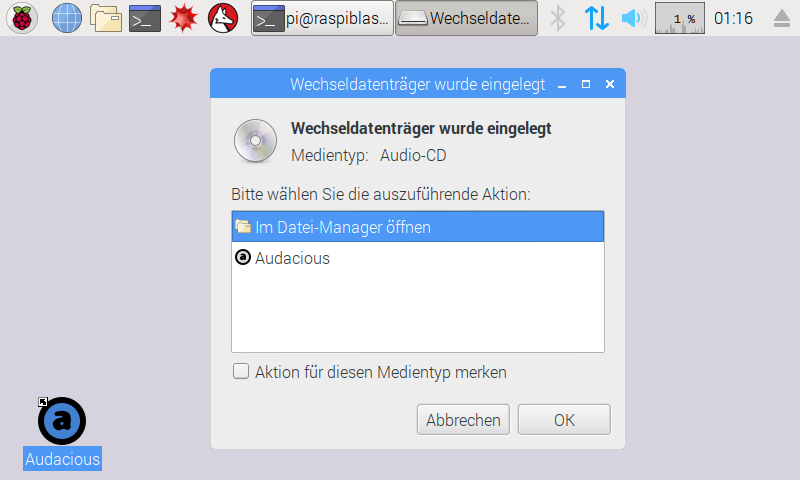
\includegraphics[width=0.8\textwidth]{\lang/desktop09.png}
\caption{Systemmeldung "`Wechseldatentr�ger wurde eingelegt"'}
\label{fig:desktop09}
\end{figure}

Das Abspielen der CD wird in {\audacious} �ber den Men�punkt 
\menuitem{Dienste$\rightarrow$CD wiedergeben} gestartet. Alle Titel der CD werden
zun�chst in eine neue Wiedergabeliste von {\audacious} mit der Bezeichnung 
"`Momentane Wiedergabeliste"' eingetragen. Wenn diese Liste bereits Musiktitel 
enth�lt, so werden alle vorhandenen Titel in dieser Liste gel�scht und mit den
Titeln der eingelegten CD ersetzt! Details siehe Abschnitt \ref{sect:playlist}.
CDs nach der urspr�nglichen CDDA-Spezifikation enthalten keine Metadaten mit 
Songtiteln, K�nstlern etc. Die Liste wird daher mit den Standardbezeichnungen 
"`Titel <x>"' und der Albumbezeichnung "`Audio-CD"' belegt. Bei neueren CDs sind 
zus�tzlich Metadaten im Format "`CD-TEXT"' enthalten. Wenn das Laufwerk solche 
Daten findet, werden diese Bezeichnungen in die Wiedergabeliste �bernommen.

\begin{bclogo}[logo = \bclampe, noborder = true]{Hinweis}
Um auch bei klassischen CDs der ersten Generation automatisch Titelinformationen 
zu erhalten, ermittelt {\audacious} die Metadaten �ber die Internetdatenbank 
\textit{Compact Disc Database} (CDDB). Dabei werden die L�ngen der einzelnen 
Titel auf der CD zu CDDB gesendet und der Server sucht damit in seiner Datenbank 
nach den Klartextinformationen zu dieser CD.\\
F�r die Nutzung von CDDB muss der {\Bezeichnung} ans Internet angeschlossen 
werden!\\
\url{https://de.wikipedia.org/wiki/CDDB}
\end{bclogo}


\section{Bedienung}
Die grafische Oberfl�che des Audioplayers {\audacious} enth�lt alle 
Bedienelemente, die man von einem klassischen CD-Spieler kennt.
\subsection*{Play/Pause}
Starten und Unterbrechen der Wiedergabe
\subsection*{Skip |<<}
Titelwahl r�ckw�rts
\subsection*{Skip >>|}
Titelwahl vorw�rts
\subsection*{Vor- und R�ckspulen innerhalb eines Titels}
Das Spulen innerhalb eines Titels erfolgt unter {\audacious} durch Verschieben 
der aktuellen Position im Fortschrittsbalken, der die bereits verstrichene Zeit 
des gerade laufenden Titels anzeigt.
\begin{bclogo}[logo = \bclampe, noborder = true]{Hinweis} 
Da mit dieser Methode wirklich sehr schnell an eine bestimmte Stelle (und auch 
an den Anfang) des Titels gesprungen werden kann, springt die Schaltfl�che 
\textit{Skip |<<} \textbf{immer} zum vorhergehenden Titel und nicht wie bei 
vielen anderen CD-Spielern zum Anfang des gerade laufenden Titels!
\end{bclogo}
\subsection*{Stop}
Anhalten der Wiedergabe
\subsection*{eject}
�ffnen der CD-Schublade des Laufwerks
\begin{bclogo}[logo = \bclampe, noborder = true]{Hinweis}
Die Funktion \textit{eject} wurde von {\autor} in die f�r den {\Bezeichnung} 
vorgesehene {\RPi}-Version des Audioplayers {\audacious} implementiert.
\end{bclogo}


\section{Wiedergabeliste}
\label{sect:playlist}
{\audacious} verwaltet alle Musiktitel, die abgespielt werden sollen, in 
sogenannten Wiedergabelisten (oder auf englisch \textit{Playlists}). Dies ist 
vor allem f�r die Zusammenstellung von l�ngeren Listen mit Audiodateien von 
einem Speichermedium wie einem USB-Massenspeicher gedacht. 
In {\audacious} k�nnen mehrere Wiedergabelisten gleichzeitig ge�ffnet sein, um 
die Musik nach verschiedenen Genres (Metal, Klassik, Schlager, Volksmusik) zu
sortieren. Allerdings wird immer nur Musik aus der gerade aktivierten 
Wiedergabeliste wiedergegeben.
\begin{bclogo}[logo = \bclampe, noborder = true]{Hinweis} 
Beim Start der Wiedergabe einer CD �ber den Men�punkt 
\menuitem{Dienste$\rightarrow$CD wiedergeben} werden immer alle Titel der CD in 
die Liste "`Momentane Wiedergabe"' eingef�gt. Sollte diese Wiedergabeliste noch 
Titel enthalten, werden diese jetzt gel�scht! Auch dieser besonderen 
Wiedergabeliste k�nnen nach dem Einlesen der CD noch weitere Titel von 
USB-Laufwerken etc. hinzugef�gt werden.\\
Wird die Wiedergabeliste "`Momentane Wiedergabe"' umbenannt, so wird bei Start 
der CD-Wiedergabe �ber den Men�punkt \menuitem{Dienste$\rightarrow$CD wiedergeben} 
eine neue Wiedergabeliste mit der Bezeichnung "`Momentane Wiedergabe"' 
angelegt. 
\end{bclogo}


\section{Audiodateien von anderen Speichermedien abspielen}
{\audacious} unterst�tzt auch die Wiedergabe von Audiodateien in vielen Formaten 
wie MP3 oder FLAC, die auf einem Speichermedium wie einer Daten-CD oder einem
USB-Laufwerk abgespeichert sind. Ebenso k�nnen Mediadateien von der SD-Karte des 
{\RPi} abgespielt werden.\\
Bei Videodateien gibt {\audacious} nur den Audiokanal wieder.


\section{Behandlung und Reinigung von CDs}
\begin{compactitem}
\item{Fassen Sie die CD stets an den Kanten an, um sie sauber zu halten}
\item{Kleben Sie kein Papier oder Klebeband auf die CD}
\item{Sch�tzen Sie die CD vor starker Hitze:\\Halten Sie sie vor direkter Sonneneinstahlung und W�rmequellen wie Heizungen fern. Lassen Sie sie auch nicht in einem direkt in der Sonne parkenden Fahrzeug liegen.}
\item{Verstauen Sie die CD nach dem Anh�ren immer in ihrer CD-H�lle}
\end{compactitem}

\begin{figure}[h]
\centering
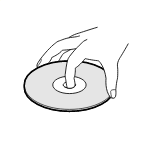
\includegraphics[width=0.3\textwidth]{CD_handling.png}
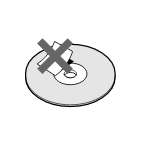
\includegraphics[width=0.3\textwidth]{CD_no_labels.png}
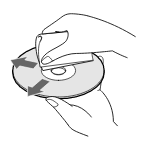
\includegraphics[width=0.3\textwidth]{CD_cleaning.png}
\caption{Behandlung von CDs}
\label{fig:CDhandling}
\end{figure}

\begin{compactitem}
\item{Reinigen Sie die CD mit einem fusselfreien Reinigungstuch und wischen Sie dabei von innen nach au�en}
\item{Verwenden Sie keine l�sungsmittelhaltigen Reinigungsmittel wie Benzin oder Verd�nner}
\end{compactitem}


\section{Fehlerbehebung}
Bei Aufreten von fehlerhaftem Verhalten des Ger�tes sollte zun�chst gepr�ft 
werden, ob der (vermeintliche) Fehler mit einfachen Mitteln zu beheben ist. 
Gerade Systeme, auf denen komplexe Software (\zB das Betriebssystem Raspbian 
oder auch {\audacious}) l�uft, sind sehr vielf�ltig konfigurierbar und nicht 
jedes unerwartete Verhalten ist wirklich ein Fehler, sondern kann oft durch 
einfache Ma�nahmen beseitigt werden.\\
Die folgende Liste erhebt keinen Anspruch auf Vollst�ndigkeit:

\subsection{Der {\Bezeichnung} bootet nicht}
\begin{compactitem}
\item{Die SD-Karte steckt nicht (mehr) richtig.}
\item{Das Dateisystem auf der SD-Karte wurde durch falsches Ausschalten besch�digt}
\item{Auf der SD-Karte wurden wider besseren Wissens ben�tigte Dateien gel�scht oder verschoben}
\end{compactitem}
In all diesen F�llen muss das Geh�use des {\Bezeichnung}s ge�ffnet werden, um 
die SD-Karte des {\RPi} entnehmen zu k�nnen, da der {\RPi} davon nicht mehr 
booten kann. Im Zweifelsfalle muss die SD-Karte an einem externen PC korrigiert 
oder neu bespielt werden!

{\begin{bclogo}[arrondi = 0.2, logo = \bcdanger, ombre = true, epOmbre = 0.25, couleurOmbre = red!75,blur]{Gefahr!} 
Vor dem �ffnen des Ger�tes muss der Netzstecker gezogen werden!\\
Ansonsten besteht die Gefahr eines gef�hrlichen Stromschlages.
\end{bclogo}


\subsection{Die Auswurftaste am {\CDROM}-Laufwerk reagiert nicht}
\begin{compactitem}
\item{W�hrend eine CD wiedergegeben wird, ist die Auswurftaste des Laufwerks gesperrt}
\end{compactitem}
Vor dem Auswurf der CD muss in {\audacious} die Schaltfl�che \button{Stop} 
bet�tigt werden, um die Wiedergabe zu beenden. Erst dann bewirkt die Bet�tigung 
der Auswurftaste das �ffnen des Laufwerks.
\begin{bclogo}[logo = \bclampe, noborder = true]{Hinweis}
Die Schaltfl�che \button{eject} in {\audacious} erm�glicht \textit{jederzeit} 
das �ffnen des {\CDROM}-Lauf\-werks.
\end{bclogo}


\subsection{Der Bildschirm ist dunkel}
\begin{compactitem}
\item{Ist der Bildschirmschoner aktiv?\\
      Eine Ber�hrung des Displays zeigt das Bild wieder an}
\item{Ist die Stromzufuhr in Ordnung, stecken die Kabel richtig?}
\item{Sind die Feinsicherungen am Netzschalter in Ordnung?}
\end{compactitem}
�berpr�fung der Netzleitung auf festen Sitz.\\
Liefert die Geb�udesteckdose wirklich Netzspannung?\\
�berpr�fung der Feinsicherungen im {\Bezeichnung}. Die Absicherung des Ger�tes 
ist zwingend zweipolig vorzunehmen!

{\begin{bclogo}[arrondi = 0.2, logo = \bcdanger, ombre = true, epOmbre = 0.25, couleurOmbre = red!75,blur]{Gefahr!} 
Vor der Kontrolle der Sicherungen muss der Netzstecker gezogen werden, selbst
wenn der Netzschalter des Ger�tes auf 0 steht! Bei ge�ffneter 
Sicherungshalterung besteht die Gefahr eines gef�hrlichen Stromschlages durch 
Ber�hrung der Kontakte!
\end{bclogo}

\begin{bclogo}[arrondi = 0.2, logo = \bcinfo, ombre = true, epOmbre = 0.25, couleurOmbre = black!30,blur]{Achtung}
Beim Wechsel der Feinsicherungen muss darauf geachtet werden, nur Sicherungen des
gleichen Typs zu verwenden:\\
max. 250V, 1A tr�ge\\
\end{bclogo}


\subsection{Kein Ton}
\begin{compactitem}
\item{Ist die Lautst�rke richtig eingestellt? \\
      Ein mit einem roten \textcolor{red}{\texttt{x}} markiertes 
      Lautsprechersymbol zeigt eine stummgeschaltete Wiedergabe an.}
\item{Leise Passage oder v�llige Stille auf der CD?}
\item{l�uft die CD wirklich?}
\item{Sind die Audioquellen (CD, USB-Stick) der in der Wiedrgabeliste aufgef�hrten Titel noch vorhanden?}
\item{Ist die CD fehlerhaft oder zu stark verkratzt?\\
      Abhilfe schafft ein Test mit einer anderen CD}
\item{Bei Verwendung externer Lautsprecher: Sind die Lautsprecher richtig 
      angeschlossen?\\
      Neben einer korrekten Verkabelung am Lautsprecheranschluss ist auf die 
      richtige Schalterstellung des Lautsprecherschalters auf der Oberseite des 
      {\Bezeichnung}s zu achten. Zur Gegenprobe den Schalter in Stellung I 
      bringen. In dieser Schalterstellung erfolgt die Audiowiedergabe �ber die 
      eingebauten Lautsprecher.}
\end{compactitem}

% chapter3.tex -- de (German)
\chapter{Installation und Konfiguration}

In diesem Kapitel wird die Installation des Betriebssystems und aller Teile der 
Software beschrieben. Ein Schwerpunkt liegt auf der Einrichtung der Toolchain 
zum Kompilieren der Open-Source-Software {\audacious} auf dem {\RPi}.

{\begin{bclogo}[arrondi = 0.2, logo = \bcdanger, ombre = true, epOmbre = 0.25, couleurOmbre = red!75,blur]{Gefahr!} 
Ein Teil der in diesem Kapitel beschriebenen Ma�nahmen erfordert das �ffnen des 
Geh�uses des {\Bezeichnung}s, um an die SD-Karte des eingebauten {\RPi} zu 
gelangen. Um beim Hantieren im Inneren des Ger�tes gef�hrliche Stromschl�ge zu 
vermeiden, muss vor dem �ffnen unbedingt der Netzstecker gezogen werden! 
\end{bclogo}

\begin{bclogo}[logo = \bclampe, noborder = true]{Hinweis}
Dieses Tutorial wurde auf dem {\RPi} unter \cmd{Linux raspiblaster 4.14.30-v7+ 
\#1102 SMP Mon Mar 26 16:45:49 BST 2018 armv7l GNU/Linux} durchgef�hrt.

Am PC weichen die Kommandos je nach verwendetem Betriebssystem (Linux oder 
Windows) voneinander ab. Auf die Unterschiede wird an den jeweiligen Stellen 
eingegangen.
\end{bclogo}

Viele Kommandos m�ssen in der folgenden Anleitung sowohl auf dem {\RPi} als 
auch auf einem PC in einem Terminalfenster eingegeben werden. Um die Daten vom 
PC auf den {\Bezeichnung} kopieren zu k�nnen, m�ssen beide Rechner am LAN (oder 
WLAN) h�ngen. Der Datenaustausch erfolgt dabei �ber \textit{ssh 
(\textbf{s}ecure \textbf{sh}ell)}.\\
Anstatt alle Kommandos am {\RPi} �ber eine zweite USB-Tastatur einzugeben, ist 
es sinnvoll, am PC ein Terminalfenster zu �ffnen, auf dem man mit \textit{ssh} 
eine Verbindung zum {\RPi} aufbaut und alle Tastatureingaben am PC erledigt. 
Dies hat vor allem den Vorteil, dass man am PC die Kommandos f�r den {\RPi} aus 
diesem PDF-Dokument mit \textit{Copy+Paste} herauskopieren und im 
ssh-Ter\-mi\-nal\-fens\-ter direkt einf�gen kann.\\
Nur der erste Teil dieses Tutorials ("`raspi-config"') kann nicht 
\textit{remote} ausgef�hrt werden, da \textit{ssh} erst auf dem {\RPi} 
aktiviert werden muss und somit vorher kein Verbindungsaufbau vom PC aus 
m�glich ist.


\newpage
\begin{bclogo}[logo = \bclampe, noborder = true]{Hinweis}
Unter Windows ist \textit{ssh} standardm��ig nicht installiert. Bei Verwendung 
eines PCs mit diesem Betriebssystem, muss zuerst das Softwarepaket 
\textit{PuTTY} installiert werden, um sich vom PC aus auf dem {\RPi} �ber 
\textit{ssh} einloggen zu k�nnen.\\
Der Download kann von der Seite \url{https://putty.org/} gestartet werden:\\
\url{https://www.chiark.greenend.org.uk/~sgtatham/putty/latest.html}

Der Verbindungsaufbau zum {\RPi} erfolgt durch Start �ber den Eintrag 
\mbox{"`PuTTY64"'} im Windows-Startmen�. Der Login erfolgt �ber die 
IP-Adresse und die Benutzerkennung \cmd{pi} samt Passwort (siehe Abbildungen 
\ref{fig:putty01} und \ref{fig:putty02}).
\end{bclogo}

\begin{figure}[h]
\centering
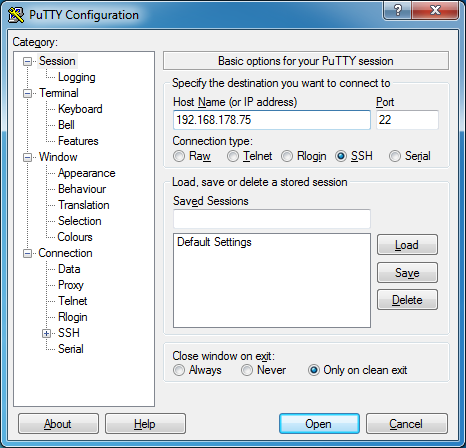
\includegraphics[width=0.5\textwidth]{putty01.png}
\caption{Verbindungsaufbau vom Windows-PC zum {\RPi} �ber \textit{PuTTY}}
\label{fig:putty01}
\end{figure}

\begin{figure}[h]
\centering
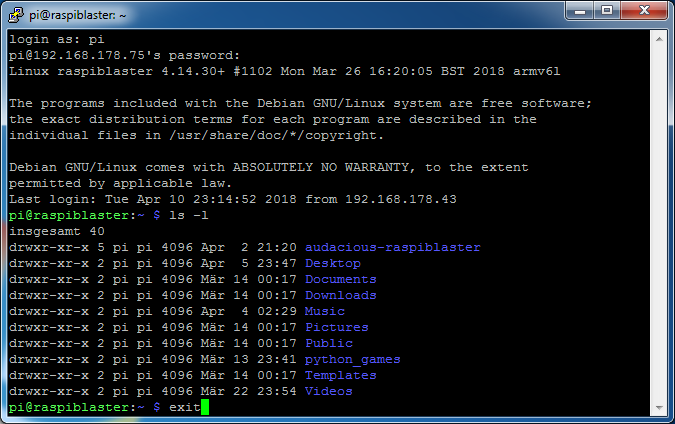
\includegraphics[width=0.75\textwidth]{putty02.png}
\caption{\textit{PuTTY}-Remote-Konsole des {\RPi} auf dem Windows-PC}
\label{fig:putty02}
\end{figure}


\newpage
\section{Raspbian einrichten}
\subsection*{raspi-config}
\cmdPi{sudo raspi-config}\\
\stdout{1 Change User Password \ \ \ \ \ \ \ \ \ \ \ \ \ \ \ \ \ \ \ \ \ \ \ \ \ \ \ }\comment{\zB "raspiBlaster"}\\
\stdout{2 Network Options \ \ \ \ \ --> N1 Hostname \ \ \ \ \ \ \ \ \ \ \ \ }\comment{"raspiblaster"\ anstatt "raspberrypi"}\\
\stdout{4 Localisation Options --> I1 Change Locale}\\
\stdout{\textcolor{white}{......................} --> I2 Change Timezone}\\
\stdout{\textcolor{white}{......................} --> I3 Change Keyboard Layout}\\
\stdout{\textcolor{white}{......................} --> I4 Change Wi-fi Country }\comment{diese Anpassung ist ganz wichtig!}\\
\stdout{5 Interfacing Options \ --> P2 SSH}

\subsection*{System aktualisieren}
\cmdPi{sudo apt update }\comment{aktualisiert nur die Metadaten}\\
\cmdPi{sudo apt upgrade}\comment{Upgrade aller installierten Pakete}\\
\cmdPi{sudo apt update }\comment{braucht's manchmal, z.B. beim verwendeten Raspbian-Image vom 13.03.2018}\\

\subsection*{Image auf ca. 6,8GB verkleinern}
TODO:\todo{entweder mein Verfahren oder \cmd{pishrink} einbinden}

Dieser Schritt ist nicht zwingend notwendig, allerdings bietet er zwei Vorteile:
\begin{compactitem}
\item{Das Image ist damit klein genug, um auf \textit{jede} 8GB-SD-Karte zu passen}
\item{Beim Sichern und Flashen von SD-Karten dauert es nicht ganz so lange}
\end{compactitem}

\subsection*{Bildausrichtung des original \raspidisplay}
Die Ausrichtung sollte um 180� gedreht werden, da dies vom Blickwinkel her besser
ist. In der Datei \filenam{/boot/config.txt} muss die Zeile \cmd{lcd\_rotate=2}
erg�nzt werden.

\cmdPi{sudo nano /boot/config.txt}\\
\editor{lcd\_rotate=2}

\subsection*{Anpassung des Raspbian-PIXEL-Desktops}
\uline{Aussehen anpassen:} \comment{reine Geschmackssache}\\
Men�punkt \menuitem{\rpiIcon$\rightarrow$Einstellungen$\rightarrow$Appearance Settings: Tab'Desktop'}\\
Checkbox \checkbox{Wastebasket} ausschalten \comment{brauchen Kinder nicht}\\
Combobox \combobox{Layout}{Centre image on screen}\\
Combobox \combobox{Picture}{raspberry-pi-logo.png} \comment{Die Himbeere als Desktopbild festlegen}

\uline{Doppelklickgeschwindigkeit verringern:}\\
Men�punkt \menuitem{\rpiIcon$\rightarrow$Einstellungen$\rightarrow$Tastatur und Maus: Tab'Maus'}\\
Schieberegler \checkbox{Double-click Delay}: \cmd{1990}ms \comment{oder so, 250ms ist am Touchdisplay sehr kurz}

\uline{Bildschirmschoner ausschalten:} \comment{optional!}\\
Folgende Zeile unter \cmd{[Seat: *]} einf�gen:

\cmdPi{sudo nano /etc/lightdm/lightdm.conf}\\
\editor{[Seat: *]\\xserver-command=X -s 0 -dpms}


\section{HiFiBerry MiniAmp installieren}
\uline{Quellen:}\\
\url{https://www.hifiberry.com/shop/boards/miniamp}\\
\url{https://www.hifiberry.com/build/documentation/configuring-linux-3-18-x}\\
\url{https://support.hifiberry.com/hc/en-us/articles/205377202-Adding-software-volume-control}

\begin{bclogo}[logo = \bclampe, noborder = true]{Hinweis}
Das Modul HiFiBerry MiniAmp V1.0 muss treiberm��ig wie ein HiFiBerry DAC 
behandelt werden!
\end{bclogo}

\subsection*{\filenam{/boot/config.txt} bearbeiten}
Entfernen des Eintrages f�r das onboard-Soundmodul (Klinke und HDMI):\\
Auskommentieren oder L�schen des Eintrages \cmd{dtparam=audio=on},\\
stattdessen "Device Tree Overlay File" f�r MiniAmp laden:

\newpage
\cmdPi{sudo nano /boot/config.txt}\\
\editor{\#dtparam=audio=on\\\vdots\\dtoverlay=hifiberry-dac}

\subsection{ALSA konfigurieren �ber \filenam{/etc/asound.conf}}
\begin{bclogo}[logo = \bclampe, noborder = true]{Hinweis}
Es ist zu �berpr�fen, ob im Homeverzeichnis des Benutzers \cmd{pi} die Datei
\filenam{.asoundrc} vorliegt. Dies ist eine Datei, die benutzerspezifische 
ALSA-Einstellungen enth�lt und die Einstellungen von 
\filenam{/etc/asound.conf} �berb�gelt!
\end{bclogo}
\cmdPi{rm /home/pi/.asoundrc}

\uline{Urspr�nglicher Inhalt von \filenam{/etc/asound.conf}:}\\
\cmdPi{cat /etc/asound.conf}\\
\stdout{pcm.!default \{}\\
\stdout{\ \ type hw card 0}\\
\stdout{\}}\\
\stdout{ctl.!default \{}\\
\stdout{\ \ type hw card 0}\\
\stdout{\}}

\cmdPi{reboot}\\
\cmdPi{aplay -l}\\
\stdout{**** Liste der Hardware-Ger�te (PLAYBACK) ****}\\
\stdout{\smaller{Karte 0: sndrpihifiberry [snd\_rpi\_hifiberry\_dac], Ger�t 0: HifiBerry DAC HiFi pcm5102a-hifi-0 []}}\\
\stdout{\ \ Sub-Ger�te: 0/1}\\
\stdout{\ \ Sub-Ger�t \#0: subdevice \#0}

\subsection{ALSA f�r Lautst�rkeregelung aufbohren}
\uline{erweiterter Inhalt von \filenam{/etc/asound.conf}:}\\
\cmdPi{cat /etc/asound.conf}\\
%\stdout{\# Einstellungen von @smutbert aus dem deutschen RaspberryPi-Forum:}\\
%\stdout{\# \url{https://forum-raspberrypi.de/user/21740-smutbert/}}\\
%\stdout{pcm.dmixer \{}\\
%\stdout{    type dmix}\\
%\stdout{    ipc\_key 1236}\\
%\stdout{    slave.pcm "hw:sndrpihifiberry"}\\
%\stdout{\}}\\
%\stdout{pcm.softvolume \{}\\
%\stdout{    type softvol}\\
%\stdout{    slave.pcm "dmixer"}\\
%\stdout{    control.name "Master"}\\
%\stdout{    control.card sndrpihifiberry}\\
%\stdout{\}}\\
%\stdout{pcm.!default \{}\\
%\stdout{    type       plug}\\
%\stdout{    slave.pcm  "{softvolume}"}\\
%\stdout{\}}
\verb|# Einstellungen von @smutbert aus dem deutschen RaspberryPi-Forum:|\\
\verb|# https://forum-raspberrypi.de/user/21740-smutbert/|\\
\verb|pcm.dmixer {|\\
\verb|    type dmix|\\
\verb|    ipc_key 1236|\\
\verb|    slave.pcm "hw:sndrpihifiberry"|\\
\verb|}|\\
\verb|pcm.softvolume {|\\
\verb|    type softvol|\\
\verb|    slave.pcm "dmixer"|\\
\verb|    control.name "Master"|\\
\verb|    control.card sndrpihifiberry|\\
\verb|}|\\
\verb|pcm.!default {|\\
\verb|    type       plug|\\
\verb|    slave.pcm  "softvolume"|\\
\verb|}|

\begin{bclogo}[logo = \bclampe, noborder = true]{Hinweis zum \textit{omxplayer}}
Die obige von \textit{@smutbert} bereitgestellte Version der 
\filenam{/etc/asound.conf} erm�glicht �ber die Definition von \textit{pcm.dmixer}
das gleichzeitige Abspielen von mehreren Audioquellen.\\
Leider funktioniert diese Variante mit dem \textit{omxplayer} nicht: Die
Mediadatei bleibt sofort bei 0:00 stehen! Der \textit{omxplayer} kann jedoch
durch zweimaliges Dr�cken von \textit{Ctrl-C} beendet werden, die Anzeige
\texttt{have a nice day ;)} erscheint allerdings nicht, da der \textit{omxplayer}
anscheinend irgendwo h�ngt\dots

Es gibt hier leider nur die beiden sich gegenseitig ausschlie�enden M�glichkeiten:\\
1. saubere ALSA-Konfiguration mit Mixerfunktionalit�t, aber kein \textit{omxplayer}!\\
2. \textit{omxplayer} mit einfacherer(?) ALSA-Konfiguration ohne Mixer verwenden.
\end{bclogo}

%\stdout{\# ab hier alter Inhalt:}\\
%\stdout{\#\#pcm.!default \{}\\
%\stdout{\#\# type hw card 0}\\
%\stdout{\#\#\}}\\
%\stdout{\#\#ctl.!default \{}\\
%\stdout{\#\# type hw card 0}\\
%\stdout{\#\#\}}\\
%\stdout{\#}\\
%\stdout{\#pcm.hifiberryMiniAmp \{}\\
%\stdout{\#    type softvol}\\
%\stdout{\#    slave.pcm "plughw:0"}\\
%\stdout{\#    control.name "Master"}\\
%\stdout{\#    control.card 0}\\
%\stdout{\#\}}\\
%\stdout{\#pcm.!default \{}\\
%\stdout{\#    type       plug}\\
%\stdout{\#    slave.pcm  "hifiberryMiniAmp"}\\
%\stdout{\#\}}
\verb|# Einstellungen ohne Mixerfunktionalit�t:|\\
\verb|# Diese Variante nur verwenden, wenn auf dem Raspiblaster der omxplayer|\\
\verb|# verwendet wird.|\\
\verb|pcm.hifiberryMiniAmp {|\\
\verb|    type softvol|\\
\verb|    slave.pcm "plughw:0"|\\
\verb|    control.name "Master"|\\
\verb|    control.card 0|\\
\verb|}|\\
\verb|pcm.!default {|\\
\verb|    type       plug|\\
\verb|    slave.pcm  "hifiberryMiniAmp"|\\
\verb|}|


\newpage
\cmdPi{rm /home/pi/.asoundrc}\\
\cmdPi{reboot}\\
\cmdPi{speaker-test -c 2}\comment{speaker-test -D hifiberryMiniAmp -c 2}\\
\cmdPi{alsamixer}

\begin{figure}[h]
\centering
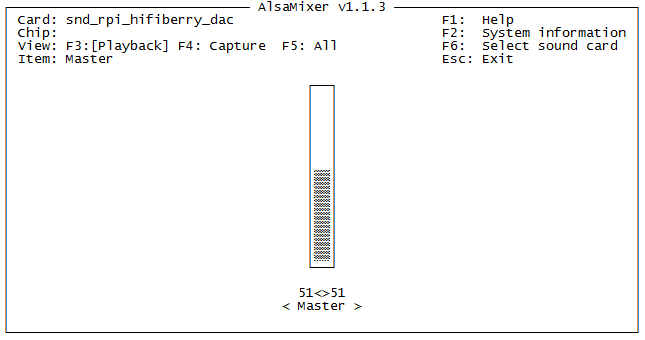
\includegraphics[width=0.8\textwidth]{\lang/alsamixer.png}
\caption{alsamixer, ein Audiomixer f�r die Konsole}
\label{fig:alsamixer}
\end{figure}

Im \textit{alsamixer} wird der in \filenam{/etc/asound.conf} definierte Regler \textit{Master} angezeigt.
\begin{bclogo}[logo = \bclampe, noborder = true]{Hinweis}
Die Lautst�rke kann jetzt �ber ALSA geregelt werden!\\
\textit{alsamixer} greift auf die gleiche Audioeinstellung zu wie der 
Lautst�rkeregler in der Taskleiste von Raspbian Desktop PIXEL.
\end{bclogo}

%% Aug. 11th 2018: Don't show the omxplayer command because it doesn't work properly on ALSA mixer definitions!
%\uline{Test:}\\
%\cmdPi{omxplayer -o alsa "01 Saga - Wind Him Up.wav"}


\section{{\CDROM}-Laufwerk am {\RPi} in Betrieb nehmen}
Wenn eine Audio-CD in das externe CD-ROM-Laufwerk (bzw. DVD-Brenner) eingelegt
wird, so wird sein Inhalt \textit{nicht} unter \filenam{/media/pi/<volume>} 
gemountet! Vielmehr wird ein virtueller(?) Ordner (bzw. eine URL) ge�ffnet: 
\cmd{cdda://sr0/}\\
Ein direkter Dateizugriff darauf ist nicht m�glich. Auch der \textit{omxplayer} 
kann diesbez�glich nicht zaubern.\\
\textbf{$\Rightarrow$ Es muss ein Software-CD-Player her!}

\newpage
\subsection{Erkennen des externen {\CDROM}-Laufwerks am USB-Anschluss}
\cmdPi{lsusb}\comment{{\CDROM}-Laufwerk nicht mit USB verbunden}\\
\stdout{\smaller{Bus 001 Device 003: ID 0424:ec00 Standard Microsystems Corp. SMSC9512/9514 Fast Ethernet Adapter}}\\
\stdout{\smaller{Bus 001 Device 002: ID 0424:9514 Standard Microsystems Corp. SMC9514 Hub}}\\
\stdout{\smaller{Bus 001 Device 001: ID 1d6b:0002 Linux Foundation 2.0 root hub}}\\
\cmdPi{lsusb}\comment{{\CDROM}-Laufwerk angesteckt}\\
\stdout{\smaller{\textcolor{darkblue}{Bus 001 Device 006: ID 0e8d:1887 MediaTek Inc.}}}\\
\stdout{\smaller{Bus 001 Device 003: ID 0424:ec00 Standard Microsystems Corp. SMSC9512/9514 Fast Ethernet Adapter}}\\
\stdout{\smaller{Bus 001 Device 002: ID 0424:9514 Standard Microsystems Corp. SMC9514 Hub}}\\
\stdout{\smaller{Bus 001 Device 001: ID 1d6b:0002 Linux Foundation 2.0 root hub}}

\subsection{Linux-Paket \textit{eject} installieren}
\label{sect:eject}
Zum �ffnen der Schublade des CD-Laufwerks ist das Programmpaket \textit{eject} 
erforderlich, das im Gegensatz zu einem normalen PC/Laptop auf dem {\RPi} unter 
Raspbian nicht installiert ist:

\cmdPi{sudo apt install eject}\comment{49,5kB Archive, 225kB Plattenplatz entpackt}\\
\cmdPi{eject \ \ }\comment{Auswurf des CD-Laufwerks}\\
\cmdPi{eject -t}\comment{Schlie�en des CD-Laufwerks: Wird nicht von allen Laufwerken unterst�tzt!}

%\begin{bclogo}[logo = \bclampe, noborder = true]{Hinweis}
Der Aufruf von \cmd{eject -t} kann verwendet werden, um bei Laufwerken, die 
diese Funktion nicht unterst�tzen, festzustellen, ob dessen Schublade ge�ffnet 
oder geschlossen \textbf{ist}. Falls ge�ffnet liefert \cmd{eject -t} eine 
Fehlermeldung und den Exitcode 1.
%\end{bclogo}

Das Kommando \cmd{eject -i 1} verhindert entgegen der Dokumentation in der 
\cmd{man}-Page (zumindest beim verwendeten Laufwerk {\LGdrive} \textbf{nicht}, 
dass das Laufwerk �ber die Auswurftaste ge�ffnet werden kann! \\
Das {\CDROM}-Laufwerk meines Laptops verh�lt sich sich genauso.


\section{\textit{audacious} auf dem {\RPi} kompilieren}
\label{sect:compile}
Erste Tests mit verschiedenen Audio- bzw. Mediaplayern ergab, dass die 
Bet�tigung der Auswurftaste des {\CDROM}-Laufwerks zu hartn�ckigen Aufh�ngern 
f�hrt, wenn gerade eine CD wiedergegeben wird, egal mit welchem Audioplayer 
die Wiedergabe erfolgt. Selbst das Kommando \cmd{sudo kill -9 <prozess-ID>}, 
bei dem alle betriebssystemseitigen Register gezogen werden, kann den h�ngenden 
Prozess nicht sauber beenden!\\
Der erste L�sungsansatz war, mit dem Kommando \cmd{eject -i 1} das �ffnen 
der Laufwerksschublade bei Druck auf die Auswurftaste zu verhindern. Aber wie 
im vorigen Kapitel (Abschnitt \ref{sect:eject}) beschrieben, bei�t dieses 
Kommando (zumindest beim verwendeten Laufwerk \LGdrive) nicht an. Daher wurde 
im verwendeten Laufwerk der Stromkreis der Auswurftaste unterbrochen und kann 
�ber ein Relais geschlossen werden, so dass die erforderliche "`eject-Sperre"' 
hardwarem��ig erfolgt und mit dem GPIO4 gesteuert werden kann.\\
Daraus resultierte die Notwendigkeit, eine Auswurffunktionalit�t inklusive 
der beschriebenen Sperre in den verwendeten Audioplayer zu implementieren. 
Hierf�r muss der Quellcode entsprechend angepasst und neu kompiliert werden.


\subsection{Download und Entpacken des aktuellen Quellcodes}
Zun�chst wurde von der {\audacious}-Homepage die Version {\audaciousStable} 
heruntergeladen. Sie besteht aus den drei Teilprojekten, die jeweils als
gepacktes \cmd{tar}-Archiv (ein sogenannter \textit{Tarball}) vorliegen:
\begin{compactitem}
\item{\cmd{libaudclient-3.5-rc2.tar.bz2}}
\item{\cmd{audacious-3.9.tar.bz2}}
\item{\cmd{audacious-plugins-3.9.tar.bz2}}
\end{compactitem}

\uline{Quellen:}\\
\url{https://audacious-media-player.org/download}

\url{https://distfiles.audacious-media-player.org/libaudclient-3.5-rc2.tar.bz2}\\
\url{https://distfiles.audacious-media-player.org/audacious-3.9.tar.bz2}\\
\url{https://distfiles.audacious-media-player.org/audacious-plugins-3.9.tar.bz2}

Davon ausgehend, dass der Download auf einem (Linux-)PC erfolgte, m�ssen diese
drei Tarballs zun�chst per \textit{ssh} auf den {\RPi} in das Verzeichnis 
\cmd{/home/pi/audacious\_raspiblaster} kopiert werden:

\cmdPi{cd /home/pi}\\
\cmdPi{mkdir audacious\_raspiblaster}

\cmdPC{scp *.tar.bz2 pi@raspiblaster:/home/pi/audacious\_raspiblaster}\\
Am PC erfolgt eine Passwortabfrage f�r den Benutzer \cmd{pi} auf dem Host
\cmd{raspiblaster}. Nur bei richtiger Eingabe k�nnen die Dateien per 
\textit{ssh}-Protokoll vom PC auf den {\RPi} �bertragen werden.

\begin{bclogo}[logo = \bclampe, noborder = true]{Hinweis}
An einem Windows-PC, auf dem die \textit{ssh}-Software \textit{PuTTY} 
installiert ist, lautet das Kommando im Windows-Konsolenfenster 
(\cmd{cmd.exe}):\\
\cmdWin{\textcolor{red}{\textbf{p}}scp *.tar.bz2 pi@raspiblaster:/home/pi/audacious\_raspiblaster}
\end{bclogo}

\uline{Entpacken der Tarballs:}\\
\cmdPi{cd audacious\_raspiblaster}\\
\cmdPi{tar -xvf audacious-3.9.tar.bz2}\\
\cmdPi{tar -xvf audacious-plugins-3.9.tar.bz2}\\
\cmdPi{tar -xvf libaudclient-3.5-rc2.tar.bz2}


\subsection{libaudclient-3.5-rc2 kompilieren}
\cmdPi{cd /home/pi/audacious\_raspiblaster/libaudclient-3.5-rc2}\\
\cmdPi{./configure}

Das Kommando \cmd{./configure} entdeckt, dass einige Programmpakete nicht 
installiert sind:\\
\cmdPi{sudo apt install libglib2.0-dev \ \ \ }\comment{wegen Meldung: Cannot find Glib2!\\If you are using binary packages based system, check that you have the corresponding -dev/devel \mbox{packages} installed.}\\
\cmdPi{sudo apt install libdbus-1-dev \ \ \ \ }\comment{wegen Meldung: No package 'dbus-1' found}\\
\cmdPi{sudo apt install libdbus-glib-1-dev}\comment{wegen Meldung: No package 'dbus-glib-1' found}\\
\cmdPi{./configure}\\
\cmdPi{make}\comment{liefert zwar einen Schwung Warnings, kompiliert es aber dennoch vollst�ndig\dots}\\
\cmdPi{sudo make install}


\subsection{audacious-3.9 kompilieren}
\cmdPi{cd /home/pi/audacious\_raspiblaster/audacious-3.9}\\
\cmdPi{leafpad INSTALL}\comment{Anzeige der Installationsanleitung}\\
\cmdPi{./configure}

Das Kommando \cmd{./configure} entdeckt, dass einige Programmpakete nicht 
installiert sind:\\
\cmdPi{sudo apt install libglib2.0-dev \ \ \ \ \ \ \ \ }\comment{wegen Meldung: No package 'glib-2.0' found}\\
\cmdPi{sudo apt install libgtk2.0 libgtk2.0-dev}\comment{wegen Meldung: No package 'gtk+-2.0' found\\$\rightarrow$Die Installation dieser Pakete dauert auf dem {\RPi} 3B ca. 5 Minuten}

\cmdPi{./configure}\\
\cmdPi{make -j4}\comment{\cmd{-j4} bewirkt, dass auf dem {\RPi} 3B alle vier Cores verwendet werden}\\
\cmdPi{sudo make install}

Der folgende Aufruf muss wegen der grafischen Darstellung der GUI direkt auf dem
{\RPi} erfolgen. Am \textit{ssh}-Terminal auf dem PC ist er nicht m�glich!\\
\cmdPi{audacious}
%# liefert Fehlermeldung: audacious: error while loading shared libraries: libaudcore.so.5: cannot open shared object file: No such file or directory
%--> Wieder ein echtes Schmankerl:
%    Die "shared libraries" werden offenbar in /usr/lib gesucht und es hat nichts
%    mit dem Inhalt der PATH-Variablen zu tun!
%    "make install" kopiert die Libraries jedoch nach /usr/local/lib.
%    Abhilfe: 
%    \cmdPi{sudo cp  /usr/local/lib/* /usr/lib}
%
%\cmdPi{audacious}
%--> Jetzt erscheint eine vers�hnlichere Meldung:
%    ERROR plugin-init.cc:147 [start_required]: No output plugin found.
%    (Did you forget to install audacious-plugins?)
%    Abgebrochen
 

\subsection{audacious-plugins-3.9 kompilieren}
\cmdPi{cd /home/pi/audacious\_raspiblaster/audacious-plugins-3.9}\\
\cmdPi{./configure}

Das Kommando \cmd{./configure} entdeckt, dass einige Programmpakete nicht 
installiert sind:\\
\cmdPi{sudo apt install libxml2-dev}\comment{wegen Meldung: No package 'libxml-2.0' found}

Beim n�chsten \cmd{./configure}-Aufruf kommt folgende Warnung:\\
\textit{checking for libcdio >= 0.70 libcdio\_cdda >= 0.70 libcddb >= 1.2.1... no\\configure: WARNING: audio CD support disabled due to missing dependency: libcdio >= 0.70 libcdio\_cdda >= 0.70 libcddb >= 1.2.1}\\
\cmdPi{sudo apt install libcdio-dev libcdio-paranoia-dev libcddb-dev}

Ferner fehlt ein Paket f�r flac (was ich mittlerweile als wichtig empfinde):\\
\textit{checking for flac >= 1.2.1... no\\configure: error: Missing dependency for FLAC support: flac >= 1.2.1}

\cmdPi{sudo apt install libflac-dev}\\
\cmdPi{sudo apt install libogg-dev libvorbis-dev}\comment{dto. f�r die Codecs ogg vorbis}\\
\cmdPi{sudo apt install libfluidsynth-dev \ \ \ \ \ \ }\comment{dto. f�r MIDI-Plugin}\\
\cmdPi{sudo apt install libmpg123-dev \ \ \ \ \ \ \ \ \ \ }\comment{dto. f�r MP3-Codec}\\
\cmdPi{sudo apt install libfaad-dev \ \ \ \ \ \ \ \ \ \ \ \ }\comment{dto. f�r AAC-Codec}\\
\cmdPi{sudo apt install libwavpack-dev \ \ \ \ \ \ \ \ \ }\comment{dto. f�r WAV-Codec}\\
\cmdPi{\# sudo apt install libsamplerate-dev \ \ \ \ }%\comment{Wichtig f�r das Plugin Speed+Pitch: Das gef�llt Alt+Jung!}

\uline{Paket neon27 f�r  HTTP/HTTPS-Transport installieren:}\\
\cmdPi{sudo apt install libneon27-dev}

\uline{H�ssliche Warnung: ALSA ist auf dem {\Bezeichnung} f�r die Audiowiedergabe erforderlich!}\\
\textit{checking for alsa >= 1.0.16... no\\configure: WARNING: ALSA output disabled due to missing dependency: alsa >= 1.0.16}\\
\cmdPi{sudo apt install libasound2-dev}

\uline{Bibliothek "libavcodec" aus dem FFmpeg-Projekt fehlt:}\\
\textit{checking for libavcodec >= 53.40.0 libavformat >= 53.25.0 libavutil >= 51.27.0... no\\configure: error: FFmpeg is not installed or too old (required: libavcodec 53.40.0, libavformat 53.25.0, libavutil 51.27.0).  Use --with-ffmpeg=none to disable the ffaudio plugin or --with-ffmpeg=libav to use libav instead.}\\
\cmdPi{sudo apt install libavcodec-dev libavformat-dev libavutil-dev}}

\begin{bclogo}[logo = \bclampe, noborder = true]{Hinweis}
Nach der Installation all dieser Pakete fehlt zwar immer noch Etliches. Darauf
kann aber offenbar verzichtet werden, da es anscheinend nicht essentiell ist.
\end{bclogo}
\cmdPi{./configure}
\smaller{\begin{verbatim}
Configuration:

  Install path:                           /usr/local/lib/audacious
  GTK+ support:                           yes
  Qt support:                             no

  Audio Formats
  -------------
  Audio CD:                               yes
  Free Lossless Audio Codec:              yes
  Ogg Vorbis:                             yes
  MIDI (via FluidSynth):                  yes
  MPEG-1 Layer I/II/III (via mpg123):     yes
  MPEG-2/4 AAC:                           yes
  WavPack:                                yes

  External Decoders
  -----------------
  FFmpeg/Libav:                           ffmpeg
  libsndfile:                             no

  Chiptunes
  ---------
  AdLib synthesizer (adplug):             yes
  Commodore 64 audio (sid):               no
  Game Music Emu (spc, nsf, gbs, etc.):   yes
  ModPlug:                                no
  Nintendo DS audio (xsf):                yes
  PlayStation audio (psf/psf2):           yes
  Vortex Tracker (vtx):                   yes

  Other Inputs
  ------------
  Metronome:                              yes
  Tone Generator:                         yes

  Effects
  -------
  Bauer stereophonic-to-binaural (bs2b):  no
  Channel Mixer:                          yes
  Crystalizer:                            yes
  Dynamic Range Compressor:               yes
  Echo/Surround:                          yes
  Extra Stereo:                           yes
  LADSPA Host (requires GTK+):            yes
  Sample Rate Converter:                  no
  Silence Removal:                        yes
  SoX Resampler:                          no
  Speed and Pitch:                        no
  Voice Removal:                          yes

  Outputs
  -------
  Advanced Linux Sound Architecture:      yes
  Jack Audio Connection Kit:              no
  Open Sound System:                      yes
  PulseAudio:                             no
  Simple DirectMedia Layer:               no
  Sndio:                                  no
  Win32 waveOut:                          no
  FileWriter:                             yes
    -> MP3 encoding:                      no
    -> Vorbis encoding:                   yes
    -> FLAC encoding:                     yes

  Playlists
  ---------
  Cue sheets:                             no
  M3U playlists:                          yes
  Microsoft ASX (legacy):                 yes
  Microsoft ASX 3.0:                      yes
  PLS playlists:                          yes
  XML Sharable Playlist Format (XSPF):    yes

  Transports
  ----------
  FTP, SFTP, SMB (via GIO):               yes
  HTTP/HTTPS (via neon):                  yes
  MMS (via libmms):                       no

  General
  -------
  Alarm (requires GTK+):                  yes
  Ampache browser (requires Qt):          no
  Delete Files:                           yes
  GNOME Shortcuts:                        yes
  libnotify OSD:                          no
  Linux Infrared Remote Control (LIRC):   no
  MPRIS 2 Server:                         yes
  Scrobbler 2.0:                          no
  Song Change:                            yes

  GTK+ Support
  ------------
  GTK Interface:                          yes
  Winamp Classic Interface:               yes
  Album Art:                              yes
  Blur Scope:                             yes
  OpenGL Spectrum Analyzer:               no
  LyricWiki viewer:                       yes
  Playlist Manager:                       yes
  Search Tool:                            yes
  Spectrum Analyzer (2D):                 yes
  Status Icon:                            yes
  X11 Global Hotkeys:                     yes
  X11 On-Screen Display (aosd):           yes
\end{verbatim}
}
%Configuration:\\
%\\
%  Install path:                           /usr/local/lib/audacious\\
%\\
%  GTK+ support:                           yes\\
%  Qt support:                             no\\
%\\
%  Audio Formats\\
%  -------------\\
%  Audio CD:                               yes\\
%  Free Lossless Audio Codec:              yes\\
%  Ogg Vorbis:                             yes\\
%  MIDI (via FluidSynth):                  yes\\
%  MPEG-1 Layer I/II/III (via mpg123):     yes\\
%  MPEG-2/4 AAC:                           yes\\
%  WavPack:                                yes\\
%\\
%  External Decoders\\
%  -----------------\\
%  FFmpeg/Libav:                           ffmpeg\\
%  libsndfile:                             no\\
%\\
%  Chiptunes\\
%  ---------\\
%  AdLib synthesizer (adplug):             yes\\
%  Commodore 64 audio (sid):               no\\
%  Game Music Emu (spc, nsf, gbs, etc.):   yes\\
%  ModPlug:                                no\\
%  Nintendo DS audio (xsf):                yes\\
%  PlayStation audio (psf/psf2):           yes\\
%  Vortex Tracker (vtx):                   yes\\
%\\
%  Other Inputs\\
%  ------------\\
%  Metronome:                              yes\\
%  Tone Generator:                         yes\\
%\\
%  Effects\\
%  -------\\
%  Bauer stereophonic-to-binaural (bs2b):  no\\
%  Channel Mixer:                          yes\\
%  Crystalizer:                            yes\\
%  Dynamic Range Compressor:               yes\\
%  Echo/Surround:                          yes\\
%  Extra Stereo:                           yes\\
%  LADSPA Host (requires GTK+):            yes\\
%  Sample Rate Converter:                  no\\
%  Silence Removal:                        yes\\
%  SoX Resampler:                          no\\
%  Speed and Pitch:                        yes\\
%  Voice Removal:                          yes\\
%\\
%  Outputs\\
%  -------\\
%  Advanced Linux Sound Architecture:      yes\\
%  Jack Audio Connection Kit:              no\\
%  Open Sound System:                      yes\\
%  PulseAudio:                             no\\
%  Simple DirectMedia Layer:               no\\
%  Sndio:                                  no\\
%  Win32 waveOut:                          no\\
%  FileWriter:                             yes\\
%    -> MP3 encoding:                      no\\
%    -> Vorbis encoding:                   yes\\
%    -> FLAC encoding:                     yes\\
%\\
%  Playlists\\
%  ---------\\
%  Cue sheets:                             no\\
%  M3U playlists:                          yes\\
%  Microsoft ASX (legacy):                 yes\\
%  Microsoft ASX 3.0:                      yes\\
%  PLS playlists:                          yes\\
%  XML Sharable Playlist Format (XSPF):    yes\\
%\\
%  Transports\\
%  ----------\\
%  FTP, SFTP, SMB (via GIO):               yes\\
%  HTTP/HTTPS (via neon):                  yes\\
%  MMS (via libmms):                       no\\
%\\
%  General\\
%  -------\\
%  Alarm (requires GTK+):                  yes\\
%  Ampache browser (requires Qt):          no\\
%  Delete Files:                           yes\\
%  GNOME Shortcuts:                        yes\\
%  libnotify OSD:                          no\\
%  Linux Infrared Remote Control (LIRC):   no\\
%  MPRIS 2 Server:                         yes\\
%  Scrobbler 2.0:                          no\\
%  Song Change:                            yes\\
%\\
%  GTK+ Support\\
%  ------------\\
%  GTK Interface:                          yes\\
%  Winamp Classic Interface:               yes\\
%  Album Art:                              yes\\
%  Blur Scope:                             yes\\
%  OpenGL Spectrum Analyzer:               no\\
%  LyricWiki viewer:                       yes\\
%  Playlist Manager:                       yes\\
%  Search Tool:                            yes\\
%  Spectrum Analyzer (2D):                 yes\\
%  Status Icon:                            yes\\
%  X11 Global Hotkeys:                     yes\\
%  X11 On-Screen Display (aosd):           yes}

\normalsize{}
\uline{Kompilieren und Installieren der Plugins:}\\
\cmd{make} mit dem Kommandozeilenparameter \cmd{-j4} bewirkt, dass auf dem 
{\RPi} 3B alle vier Cores verwendet werden. Dennoch dauert der Kompiliervorgang 
damit immer noch ca. 5 Minuten:\\
\cmdPi{make -j4}\comment{\cmd{-j4} bewirkt, dass auf dem {\RPi} 3B alle vier Cores verwendet werden}\\
\cmdPi{sudo make install}

%Den folgenden Befehl braucht's (mit dem neuen Raspbian Stretch 2018-03-13?) offenbar nicht mehr...
%\cmdPi{sudo cp -r /usr/local/lib/audacious/pkgconfig /usr/local/lib/audacious/audacious /usr/local/lib/audacious/libaud* /usr/lib}\comment{{\dots}und auch hier die Bibliotheken nach /usr/lib kopieren}\\
%*** STRIKE! ***


\subsection{Code von {\audacious} auf den {\Bezeichnung} anpassen}
Um die �nderungen von {\autor} einzuspielen, muss lediglich der angepasste 
Quellcode vom GitHub-Re\-po\-si\-to\-ry 
\url{https://github.com/schlizbaeda/audacious-raspiblaster} heruntergeladen 
werden und die drei soeben erstellten \textit{audacious}-Projekte mit den 
heruntergeladenen Dateien aktualisiert und neu kompiliert werden:

\cmdPi{git clone https://github.com/schlizbaeda/audacious-raspiblaster download}\\
\cmdPi{cd /home/pi/download}\\
\cmdPi{cp -r libaudclient-3.5-rc /home/pi/audacious-raspiblaster}\\
\cmdPi{cp -r audacious-3.9 /home/pi/audacious-raspiblaster}\\
\cmdPi{cp -r audacious-plugins-3.9 /home/pi/audacious-raspiblaster}

Anschlie�end in jedem Projektverzeichnis die Projekte mit dem ge�nderten Code 
neu erstellen:\\
\cmdPi{cd /home/pi/audacious\_raspiblaster/libaudclient-3.5-rc2}\comment{dto. f�r die beiden anderen Teilprojekte}\\
\cmdPi{make -j4}\\
\cmdPi{sudo make install}

\begin{bclogo}[logo = \bclampe, noborder = true]{Hinweis}
Die vom {\autor} ge�nderten Stellen im Code sind mit dem Kommentar 
\cmd{schlizb�da} gekennzeichnet. Alle ge�nderten Dateien k�nnen mit dem 
folgenden Kommando ermittelt werden:\\
\cmdPi{cd /home/pi/audacious\_raspiblaster}\\
\cmdPi{grep -r schlizb�da *}\comment{durchsucht rekursiv alle Dateien nach dem Suchbegriff}
\end{bclogo}


\newpage
\begin{bclogo}[logo = \bclampe, noborder = true]{Hinweis}
Die folgenden Abschnitte brauchen f�r die Installation von {\audacious} auf dem 
{\RPi} nicht mehr ausgef�hrt zu werden! Sie sind hier lediglich enthalten, um 
die urspr�ngliche Vorgehensweise zu beschreiben.
\end{bclogo}

\subsection{Entwicklungsumgebung \textit{eclipse} f�r die Codeanalyse und den Debug von \textit{audacious} auf dem PC verwenden}
Zur �nderung des Sourcecodes von audacity wird ein Laptop mit Linux Mint 18.02
verwendet. Auch dort kann ein programmtechnischer Zugriff auf ein 
{\CDROM}-Lauf\-werk �hnlicher Bauart erfolgen...\\
M�glicherweise muss erst noch das Linux-Paket \cmd{eject} auf dem PC installiert
werden:\\
\cmdPC{sudo apt install eject}

\cmdPC{sudo apt install eclipse eclipse-cdt}\comment{Installation mit C-/C++-Plugin}\\
\cmdPC{eclipse \& \ \ \ \ \ \ \ \ \ \ \ \ \ \ \ \ \ \ \ \ \ \ \ \ \ \ \ \ \ \ }\comment{Start im Hintergrund}

\uline{Bestehendes Projekt in \textit{eclipse} einlesen:}\\
\menuitem{File$\rightarrow$New$\rightarrow$C++ Project}\\
Es �ffnet sich der Dialog "C++ Project". Dort VORHANDENES Projekt mit folgenden Optionen/Einstellungen einlesen:
\begin{compactitem}
\item{Project Name: \cmd{audacious}}
\item{Use default location: Das H�kchen entfernen!}
\item{Location: mit \button{Browse} das Verzeichnis w�hlen: \smaller{\filenam{/home/peter/audacious\_raspiblaster/audacious-3.9}}}
\item{Project type: Anw�hlen von \menuitem{Makefile project$\rightarrow$Empty Project}}
\item{Toolchain: Linux GCC}
\end{compactitem}
Einlesen mit der Schaltfl�che \button{Finish} ausf�hren.

\uline{Bedienung des Debuggers:}
\begin{compactitem}
\item{Mit Linksdoppelklick auf die ganz linke Leiste setzt/entfernt man einen Breakpoint}
\item{Start des Debuggers mit dem \textit{Bug}-Symbol (Krabbeltier): Es werden zus�tzliche Ansichten ge�ffnet!}
\item{F5: Einzelschritt mit Sprung in Unterbl�cke}
\item{F6: Einzelschritt komplett}
\item{F7: aktuellen Block verlassen}
\item{F8: Fortf�hren bis zum n�chsten Breakpoint (oder Programmende)}
\end{compactitem}


\subsection{�ndern/Anpassen des Sourcecodes -- Teil 1: Einbinden der \textit{eject}-Funktionalit�t}
Neue Dateien eject.cc und eject.h in .../audacious-3.9/src/libaudcore einbinden:
\begin{compactitem}
\item{\filenam{\dots/audacious-3.9/src/libaudcore/Makefile}\\
      Einf�gen der neuen Quellcodedatei im Abschnitt \cmd{SRCS}\\
      \cmd{SRCS}\\
      \editor{eject.cc}}
\item{in \filenam{\small{\dots/audacious-3.9/src/libaudcore}} die Dateien \filenam{eject.h} und \filenam{eject.cc} anlegen}
\item{\filenam{\small{\dots/audacious-3.9/src/libaudcore/eject.cc}}: Quellcode anpassen\\
      Mordsgeschiss bei den \cmd{\#include}s, \cmd{\#define}s und Funktionsprototypen (siehe Quellcode)}
\item{\filenam{\small{\dots/audacious-3.9/src/libaudcore/tests/drct.h}}: Funktionsprototypen aufgenommen\\
      \cmd{\smaller{void aud\_drct\_eject (); /* schlizb�da: click event handler of eject button */}}}
\item{\filenam{\small{\dots/audacious-plugins-3.9/src/gtkui/ui\_gtk.cc}}: ToolStripItem "{eject}"\ aufgenommen:\\
      \cmd{\smaller{toolbar\_button\_add (toolbar, aud\_drct\_eject, "media-eject"); /* schlizb�da: added "{eject}"\ button */}}}
\item{\filenam{\small{\dots/audacious-plugins-3.9/src/gtkui/menus.cc}}: Men�punkt "{eject}"\ aufgenommen\\
      \smaller{
      \cmd{static const AudguiMenuItem playback\_items[] = \{ /* schlizb�da: added "{eject}"\ menu item */}\\
      \editor{MenuCommand (N\_("Eject"), "media-eject", NONE, aud\_drct\_eject),}\\
      \stdout{\}}}}
\end{compactitem}


\subsection{�ndern/Anpassen des Sourcecodes -- Teil 2: Besonderheiten am {\RPi} \bzw {\Bezeichnung}: eject-Sperre}
Sperren der EJECT-Taste des {\CDROM}-Laufwerks �ber GPIO4 mittels der GPIO-Bibliothek \textit{wiringPi}:\\
Neue Routinen in \filenam{\dots/audacious-3.9/src/libaudcore/eject.cc}:\\
\cmd{int lock\_eject\_pushbutton()}\\
\cmd{int unlock\_eject\_pushbutton()}\\
\cmd{int lock\_eject\_raspberrypi(bool lock) \smaller{/* wird compiliert, wenn der \#define RASPBERRYPI definiert ist */}}
  
\begin{bclogo}[logo = \bclampe, noborder = true]{Hinweis}
Hier ist es wichtig, \textit{wiringPi} zu verwenden und nicht \textit{pigpio}, 
da diese Bibliothek offenbar \textbf{alle} GPIOs des {\RPi} belegt und dabei den
I2S-Bus f�r die Audioausgabe �ber den HifiBerry MiniAMP "`ausbremst"'\dots
\end{bclogo}













%%%%%%%%%%%%%%%%%%%%%%%%%%%%%%%%%%%%%%%%%%%%%%%%%%%%%%%%%%%%%%%%%%%%%%%%%%%%%%%%
%\section{CD-ROM-Laufwerk am RPi einbinden}
%\subsection{Erkennen des externen CD-ROM-Laufwerks am USB}
%\subsection{Linux-Paket "eject" installieren}
%%\subsection{audacious kompilieren (damit man den Quellcode anpassen kann)}
%
%
%\section{audacious kompilieren (damit man den Quellcode anpassen kann)}
%\subsection{Download des aktuellen Quellcodes von https://audacious-media-player.org/download}
%\subsection{libaudclient-3.5-rc2 kompilieren}
%\subsection{audacious-3.9 kompilieren}
%\subsection{audacious-plugins-3.9 kompilieren}
%\subsection{ECLIPSE auf dem PC f�r Debug verwenden}
%\subsection{�ndern/Anpassen des Sourcecodes -- Teil 1: eject-Funktionalit�t einbinden}
%\subsection{�ndern/Anpassen des Sourcecodes -- Teil 2: RPi-/Raspiblaster-Besonderheiten}
%
%
%\section{Fehlschl�ge}
%\subsection{Python-Script mit mplayer-Aufrufen}
%\subsection{alsaplayer}
%\subsection{mpd}
% nicht durchexerziert
%\subsection{KSCD}
%desastr�s!
%\subsection{\dots}
%

% chapter4.tex -- de (German)
\chapter{CDs rippen mit \textit{abcde}}

Da der {\Bezeichnung} auf dem {\RPi} 3B basiert, handelt es sich bei diesem
Ger�t um einen vollst�ndigen Computer, auf dem das Betriebssystem 
\textit{Raspbian} l�uft. Dies ist die von der Foundation gewartete offizielle
Linux-Distribution f�r den {\RPi}, die von \textit{Debian GNU/Linux} abgeleitet
wurde. Ein solcher Computer kann prinzipiell mit beliebiger zus�tzlicher 
Software erweitert werden.\\
Dieses Kapitel beschreibt die Installation und Anwendung des Programms
\textit{abcde}\\("`\textbf{A} \textbf{B}etter \textbf{CD} \textbf{E}ncoder"'),
eines CD-Rippers f�r die Kommandozeile.

\begin{bclogo}[logo = \bclampe, noborder = true]{Hinweis}
\textit{Rippen} bezeichnet das Kopieren von einer Datenquelle auf ein anderes
Speichermedium wie eine Festplatte.\\
Die rechtliche Grundlage, von einer urheberrechtlich gesch�tzten Datenquelle 
eine Kopie mit Hilfe eines Rip-Programms zu erstellen, ist weltweit uneinheitlich
geregelt. Im europ�ischen Raum gilt vielfach, dass f�r rein private Zwecke
Kopien im eingeschr�nkten Rahmen einer sogenannten \textit{Privatkopie} erlaubt
sind.\\
(Quelle: \url{https://de.wikipedia.org/wiki/Rippen})
\end{bclogo}


\section{\textit{abcde} installieren und anpassen}
Mit \textit{abcde} k�nnen Audio-CDs ausgelesen und die Tracks anschlie�end in
die Formate \textit{flac}, \textit{m4a}, \textit{mp3}, \textit{mpc},
\textit{ogg}, \textit{opus}, \textit{mka}, \textit{spx}, \textit{vorbis},
\textit{wav}, \textit{wv}, \textit{ape}, \textit{aiff} (Stand Programmversion
2.8.x) kodiert werden. Metadaten wie Interpret, Titel, Album usw. k�nnen von
den Datenbankservern \textit{Free DB (CDDB)} oder \textit{musicbrainz} 
heruntergeladen und bearbeitet werden.\\
Im Gegensatz zu vielen anderen CD-Ripper-Pro\-gram\-men ist \textit{abcde} 
eine kommandozeilenbasierende Software, von daher relativ ressourcenschonend
und somit auch f�r den {\RPi} geeignet. Die meisten Linux-Distri\-bu\-tionen 
enthalten \textit{abcde} in ihrem Paketverwaltungssystem, deshalb ist eine 
einfache Installation m�glich. Der Quellcode von \textit{abcde} befindet sich
unter \url{https://abcde.einval.com/download/}

\subsection{Installation von \textit{abcde} �ber die Raspbian-Paketverwaltung \textit{apt}}
Diese Installationsanleitung funktioniert nicht nur auf dem {\RPi}, sondern auf
allen Rechnern, auf denen eine auf \textit{Debian} basierende Linux-Distribution
installiert ist, wie \zB \textit{ubuntu} oder \textit{Linux Mint}.

\cmdPi{sudo apt-get install abcde \ \ \ }\comment{Hauptprogramm und notwendige Pakete}\\
\cmdPi{}\comment{Installation einer Auswahl g�ngiger Audiocodecs:}\\
\cmdPi{sudo apt-get install flac lame mkcue mp3gain speex vorbis-tools vorbisgain}\\
\cmdPi{sudo apt-get install id3 id3v2}\comment{ID3-Tags f�r MP3-Dateien (empfehlenswert)}\\
\cmdPi{sudo apt-get install glyrc \ \ \ }\comment{fehlt zumindest am PC bei Linux Mint 18.2}

\subsection{Anpassung der Konfigurationsdatei \filenam{/etc/abcde.conf}}
Diese Anleitung beschreibt, wie CDs im \textit{flac}-Format gerippt werden. 
Hierbei handelt es sich um einen Audiokodierer/-dekodierer, der die Audiodaten
\textbf{verlustfrei} umwandelt und lediglich komprimiert, aber keine vermeintlich
unh�rbaren Teile entfernt, um die resultierenden Dateien weiter zu verkleinern,
so wie dies beispielsweise bei \textit{Vorbis} oder \textit{MP3} als sogenannte
verlustbehaftete Audiokompression geschieht.
\begin{figure}[h]
\centering

\includegraphics[width=0.33\textwidth]{flac_logo.png}
\caption{FLAC - Free Lossless Audio Codec}
\label{fig:flac}
\end{figure}

\cmdPi{sudo nano /etc/abcde.conf}\\
\verb|# abcde.conf -- Bearbeitete Version von schlizb�da f�r den Raspiblaster|\\
\verb|#|\\
\verb|# Diese Datei enth�lt im Original sehr viele Kommentarzeilen, die mit \#|\\
\verb|# beginnen und Erl�uterungen zu den einzelnen Optionen enthalten.|\\
\verb|# Hier werden aus Platzgr�nden nur die aktiven Zeilen aufgelistet:|\\
%\verb|CDDBMETHOD=cddb,cdtext|\\ % don't use this option. It creates additional and unnecessary errors...
\verb|HELLOINFO="`whoami`@`hostname`"|\\
\verb|ACTIONS=default,playlist,getalbumart|\\
\verb|FLACOPTS=-8|\\
\verb|OUTPUTDIR=/home/`whoami`/Music|\\
\verb|OUTPUTTYPE=flac|\\
\verb|OUTPUTFORMAT='${ARTISTFILE}/${ALBUMFILE}/${TRACKNUM}_${TRACKFILE}'|\\
\verb|VAOUTPUTFORMAT='Various_Artists/${ALBUMFILE}/${TRACKNUM}_${ARTISTFILE}__${TRACKFILE}'|\\
\verb|PLAYLISTFORMAT='${ARTISTFILE}/${ALBUMFILE}/${ARTISTFILE}__${ALBUMFILE}.${OUTPUT}.m3u'|\\
\verb|VAPLAYLISTFORMAT='Various_Artists/${ALBUMFILE}/${ALBUMFILE}.${OUTPUT}.m3u'|\\
\verb|EJECTCD=y|

Auf eine Beschreibung der Optionen in den einzelnen Zeilen wird an dieser Stelle
verzichtet. Die bei der Installation von \textit{abcde} angelegte Originaldatei 
\filenam{/etc/abcde.conf} enth�lt zu jeder Option erkl�rende Kommentare.
%Mit dieser Bedienungsanleitung wurde eine Version von \filenam{abcde.conf} 
%heruntergeladene, die direkt nach \filenam{/etc} kopiert werden kann:\\
%\cmdPi{sudo cp abcde.conf /etc}\comment{Alternative zum Editieren der Konfigurationsatei}\\
\begin{bclogo}[logo = \bclampe, noborder = true]{Hinweis}
Eine Vorlage der Datei \filenam{/etc/abcde.conf} befindet sich im
Downloadbereich der Bedienungsanleitung im Unterverzeichnis \filenam{conf}
\end{bclogo}

\section{Die erste CD mit \textit{abcde} rippen}
\label{sect:rip}
Um eine CD zu rippen, legt man die gew�nschte CD zun�chst ins \CDROM-Laufwerk ein
und \textbf{wartet, bis das Laufwerk die CD erkannt hat.} Jetzt gibt man einfach 
\texttt{abcde} in das Terminalfenster ein:\\
\cmdPi{abcde}\comment{Rippen der eingelegten CD}

Alle gew�nschten Optionen wurden ja bereits in der Datei
\filenam{/etc/abcde.conf} vorgenommen.

Nach dem Programmstart wird das Inhaltsverzeichnis der CD eingelesen. Bei
vorhandenem Internetzugang wird versucht, die Metadaten f�r die CD zu ermitteln
und anzuzeigen:

\footnotesize{\color{gray}
\verb|Grabbing entire CD - tracks: 01 02 03 04 05 06 07 08 09 10 11 12 13 14 15|\\
\color{black}\verb|Which entry would you like abcde to use (0 for none)? [0-2]: |\color{red}\verb|1|\\
\color{gray}
\verb|Selected: #1 (Saga / The Very Best Of...)|\\
\verb|---- Saga / The Very Best Of... ----|\\
\verb|Year: 1994|\\
\verb|Genre: Rock|\\
\verb|1: Wind Him Up|\\
\verb|2: (You Were) Never Alone (edited version)|\\
\verb|3: Wildest Dreams|\\
\verb|4: Humble Stance|\\
\verb|5: You and the Night|\\
\verb|6: The Flyer|\\
\verb|7: The Security of Illusion|\\
\verb|8: Why Not (single edit)|\\
\verb|9: How Long|\\
\verb|10: Only Time Will Tell|\\
\verb|11: Starting All Over|\\
\verb|12: What Do I Know|\\
\verb|13: Help Me Out|\\
\verb|14: Say Goodbye to Hollywood|\\
\verb|15: On the Loose|\\
\color{black}\verb|Edit selected CDDB data [y/N]? |\color{red}\verb|n|\\
\color{black}\verb|Is the CD multi-artist [y/N]? |\color{red}\verb|n|\\
\color{gray}
\verb|Creating playlist...|\\
\verb|- Artist   : saga|\\
\verb|- Album    : the_very_best_of|\\
\verb|- Language : en|\\
\verb|- Type     : cover|\\
} % end of block \footnotesize{

\normalsize{Nun wird versucht, im Internet ein Coverbild der CD zu finden:}

\footnotesize{\color{gray}
\verb|---- Triggering: musictree local coverartarchive |\\
\verb|#[00/01] Checking image-types: [- DLError: Couldn't resolve host name [6]|\\
\verb|- DLError: Couldn't resolve host name [6]|\\
\verb|- DLError: Couldn't resolve host name [6]|\\
\verb|- DLError: Couldn't resolve host name [6]|\\
\verb|- DLError: Couldn't resolve host name [6]|\\
\verb|- DLError: Couldn't resolve host name [6]|\\
\verb|- DLError: Couldn't resolve host name [6]|\\
\verb|!!!!!!!] (-7 item(s) less)|\\
\verb|---- Triggering: lastfm jamendo musicbrainz |\\
\verb|---- Triggering: slothradio lyricswiki discogs |\\
\verb|#[00/01] Checking image-types: [.] (-0 item(s) less)|\\
\verb|---- |\\
\verb||\\
\verb|///// ITEM #1 /////|\\
\verb|WRITE to '/home/pi/abcde.f010540f/cover.jpg'|\\
\verb|FROM: <https://images-na.ssl-images-amazon.com/images/I/51pvlJE0euL.jpg>|\\
\verb|PROV: slothradio|\\
\verb|SIZE: 51017 Bytes|\\
\verb|MSUM: 73c8ac08904a48b69be23513bbd9e04c|\\
\verb|TYPE: cover|\\
\verb|SAFE: No|\\
\verb|RATE: 0|\\
\verb|STMP: 0.000000|\\
\verb|FRMT: jpeg|\\
\verb|DATA: <not printable>|\\
\verb||\\
\verb|////////////////////|\\
\verb|# => 1 item in total.|\\
\verb|/home/pi/abcde.f010540f/cover.jpg JPEG 500x500 500x500+0+0 8-bit sRGB 51KB 0.000u 0:00.000|\\
\color{black}\verb|Do you want to enter URL or local path for the album art [y/N]? |\color{red}\verb|n|\\
} % end of block \footnotesize{

\normalsize{Einlesen der einzelnen Titel der CD:}

\footnotesize{\color{gray}
\verb|Grabbing track 01: Wind Him Up...|\\
\verb|cdparanoia III release 10.2 (September 11, 2008)|\\
\verb||\\
\verb|Ripping from sector      32 (track  1 [0:00.00])|\\
\verb|	  to sector   26131 (track  1 [5:47.74])|\\
\verb||\\
\verb|outputting to /home/pi/abcde.f010540f/track01.wav|\\
\verb||\\
\verb+ (== PROGRESS == [                              | 026131 00 ] == :^D * ==)   +\\
\verb||\\
\verb|Done.|\\
\verb||\\
\verb||\\
\verb|Grabbing track 02: (You Were) Never Alone (edited version)...|\\
\verb|cdparanoia III release 10.2 (September 11, 2008)|\\
\verb||\\
\verb|Ripping from sector   26132 (track  2 [0:00.00])|\\
\verb|	  to sector   44626 (track  2 [4:06.44])|\\
\verb||\\
\verb|outputting to /home/pi/abcde.f010540f/track02.wav|\\
\verb||\\
\verb+ (== PROGRESS == [                              | 044626 00 ] == :^D * ==)   +\\
\verb||\\
\verb|Done.|\\
\verb||\\
\verb||\\
\verb|Grabbing track 03: Wildest Dreams...|\\
} % end of block \footnotesize{
\normalsize{ \ \ \vdots \ \ (Einlesen aller �brigen Titel der CD\dots)}\\
\footnotesize{\color{gray}
%cdparanoia III release 10.2 (September 11, 2008)
%
%Ripping from sector   44627 (track  3 [0:00.00])
%	  to sector   67001 (track  3 [4:58.24])
%
%outputting to /home/pi/abcde.f010540f/track03.wav
%
% (== PROGRESS == [                              | 067001 00 ] == :^D * ==)   
%
%Done.
%
%
%Grabbing track 04: Humble Stance...
%cdparanoia III release 10.2 (September 11, 2008)
%
%Ripping from sector   67002 (track  4 [0:00.00])
%	  to sector   92731 (track  4 [5:43.04])
%
%outputting to /home/pi/abcde.f010540f/track04.wav
%
% (== PROGRESS == [                              | 092731 00 ] == :^D * ==)   
%
%Done.
%
%
%Grabbing track 05: You and the Night...
%cdparanoia III release 10.2 (September 11, 2008)
%
%Ripping from sector   92732 (track  5 [0:00.00])
%	  to sector  116441 (track  5 [5:16.09])
%
%outputting to /home/pi/abcde.f010540f/track05.wav
%
% (== PROGRESS == [                              | 116441 00 ] == :^D * ==)   
%
%Done.
%
%
%Grabbing track 06: The Flyer...
%cdparanoia III release 10.2 (September 11, 2008)
%
%Ripping from sector  116442 (track  6 [0:00.00])
%	  to sector  133091 (track  6 [3:41.74])
%
%outputting to /home/pi/abcde.f010540f/track06.wav
%
% (== PROGRESS == [                              | 133091 00 ] == :^D * ==)   
%
%Done.
%
%
%Grabbing track 07: The Security of Illusion...
%cdparanoia III release 10.2 (September 11, 2008)
%
%Ripping from sector  133092 (track  7 [0:00.00])
%	  to sector  158746 (track  7 [5:42.04])
%
%outputting to /home/pi/abcde.f010540f/track07.wav
%
% (== PROGRESS == [                              | 158746 00 ] == :^D * ==)   
%
%Done.
%
%
%Grabbing track 08: Why Not (single edit)...
%cdparanoia III release 10.2 (September 11, 2008)
%
%Ripping from sector  158747 (track  8 [0:00.00])
%	  to sector  176016 (track  8 [3:50.19])
%
%outputting to /home/pi/abcde.f010540f/track08.wav
%
% (== PROGRESS == [                              | 176016 00 ] == :^D * ==)   
%
%Done.
%
%
%Grabbing track 09: How Long...
%cdparanoia III release 10.2 (September 11, 2008)
%
%Ripping from sector  176017 (track  9 [0:00.00])
%	  to sector  193831 (track  9 [3:57.39])
%
%outputting to /home/pi/abcde.f010540f/track09.wav
%
% (== PROGRESS == [                              | 193831 00 ] == :^D * ==)   
%
%Done.
%
%
%Grabbing track 10: Only Time Will Tell...
%cdparanoia III release 10.2 (September 11, 2008)
%
%Ripping from sector  193832 (track 10 [0:00.00])
%	  to sector  213501 (track 10 [4:22.19])
%
%outputting to /home/pi/abcde.f010540f/track10.wav
%
% (== PROGRESS == [                              | 213501 00 ] == :^D * ==)   
%
%Done.
%
%
%Grabbing track 11: Starting All Over...
%cdparanoia III release 10.2 (September 11, 2008)
%
%Ripping from sector  213502 (track 11 [0:00.00])
%	  to sector  231581 (track 11 [4:01.04])
%
%outputting to /home/pi/abcde.f010540f/track11.wav
%
% (== PROGRESS == [                              | 231581 00 ] == :^D * ==)   
%
%Done.
%
%
%Grabbing track 12: What Do I Know...
%cdparanoia III release 10.2 (September 11, 2008)
%
%Ripping from sector  231582 (track 12 [0:00.00])
%	  to sector  247881 (track 12 [3:37.24])
%
%outputting to /home/pi/abcde.f010540f/track12.wav
%
% (== PROGRESS == [                              | 247881 00 ] == :^D * ==)   
%
%Done.
%
%
%Grabbing track 13: Help Me Out...
%cdparanoia III release 10.2 (September 11, 2008)
%
%Ripping from sector  247882 (track 13 [0:00.00])
%	  to sector  274359 (track 13 [5:53.02])
%
%outputting to /home/pi/abcde.f010540f/track13.wav
%
% (== PROGRESS == [                              | 274359 00 ] == :^D * ==)   
%
%Done.
%
%
%Grabbing track 14: Say Goodbye to Hollywood...
%cdparanoia III release 10.2 (September 11, 2008)
%
%Ripping from sector  274360 (track 14 [0:00.00])
%	  to sector  294759 (track 14 [4:31.74])
%
%outputting to /home/pi/abcde.f010540f/track14.wav
%
% (== PROGRESS == [                              | 294759 00 ] == :^D * ==)   
%
%Done.
%
%
\verb|Grabbing track 15: On the Loose...|\\
\verb|cdparanoia III release 10.2 (September 11, 2008)|\\
\verb||\\
\verb|Ripping from sector  294760 (track 15 [0:00.00])|\\
\verb|	  to sector  313556 (track 15 [4:10.46])|\\
\verb||\\
\verb|outputting to /home/pi/abcde.f010540f/track15.wav|\\
\verb||\\
\verb+ (== PROGRESS == [                              | 313556 00 ] == :^D * ==)   +\\
\verb||\\
\verb|Done.|\\
\verb||\\
\verb||\\
\verb|Encoding track 15 of 15: On the Loose...|\\
\verb|Tagging track 15 of 15: On the Loose...|\\
\verb|Finished.|\\
} % end of block \footnotesize{

\normalsize{Die von der CD gerippten Musikst�cke werden nach folgendem Schema in
das Verzeichnis \texttt{/home/\textit{<Benutzername>}/Music} kopiert:\\
\texttt{/home/\textit{<Benutzername>}/Music/\textit{<Interpret>}/\textit{<Album>}}\\
\texttt{/home/\textit{<Benutzername>}/Music/Various\_Artists/\textit{<Album>}}

Die soeben von der CD "`{Saga -- The Very Best Of...}"' gerippten Musiktitel
werden also im Verzeichnis \texttt{/home/pi/Music/Saga/The\_Very\_Best\_Of...}
abgelegt:

\cmdPi{ls -l /home/pi/Music/Saga/The\_Very\_Best\_Of...}\\
\stdout{total 482504}\\
\stdout{-rw-r--r-- 1 pi pi 41920468 Aug 11 12:58 01\_Wind\_Him\_Up.flac}\\
\stdout{-rw-r--r-- 1 pi pi 30166196 Aug 11 12:58 02\_(You\_Were)\_Never\_Alone\_(edited\_version).flac}\\
\stdout{-rw-r--r-- 1 pi pi 35710370 Aug 11 12:59 03\_Wildest\_Dreams.flac}\\
\stdout{-rw-r--r-- 1 pi pi 36649779 Aug 11 12:59 04\_Humble\_Stance.flac}\\
\stdout{-rw-r--r-- 1 pi pi 34147496 Aug 11 13:00 05\_You\_and\_the\_Night.flac}\\
\stdout{-rw-r--r-- 1 pi pi 28216453 Aug 11 13:00 06\_The\_Flyer.flac}\\
\stdout{-rw-r--r-- 1 pi pi 39326472 Aug 11 13:01 07\_The\_Security\_of\_Illusion.flac}\\
\stdout{-rw-r--r-- 1 pi pi 30377630 Aug 11 13:02 08\_Why\_Not\_(single\_edit).flac}\\
\stdout{-rw-r--r-- 1 pi pi 26811872 Aug 11 13:02 09\_How\_Long.flac}\\
\stdout{-rw-r--r-- 1 pi pi 31983909 Aug 11 13:03 10\_Only\_Time\_Will\_Tell.flac}\\
\stdout{-rw-r--r-- 1 pi pi 26682581 Aug 11 13:03 11\_Starting\_All\_Over.flac}\\
\stdout{-rw-r--r-- 1 pi pi 26878160 Aug 11 13:03 12\_What\_Do\_I\_Know.flac}\\
\stdout{-rw-r--r-- 1 pi pi 42271986 Aug 11 13:04 13\_Help\_Me\_Out.flac}\\
\stdout{-rw-r--r-- 1 pi pi 31089476 Aug 11 13:04 14\_Say\_Goodbye\_to\_Hollywood.flac}\\
\stdout{-rw-r--r-- 1 pi pi 31753532 Aug 11 13:04 15\_On\_the\_Loose.flac}\\
\stdout{-rw-r--r-- 1 pi pi \ \ \ 51017 Aug 11 12:57 cover.jpg}\\
\stdout{-rw-r--r-- 1 pi pi \ \ \ \ \ 388 Aug 11 12:56 Saga\_\_The\_Very\_Best\_Of....flac.m3u}

Neben den Musikdateien der 15 Titel der CD, die in das verlustfreie flac-Format
gewandelt wurden, befindet sich in diesem Verzeichnis eine \textit{m3u}-Datei
mit allen Liedern der CD. Diese Datei kann von vielen Audio-Wiedergabeprogrammen
sowohl unter Linux als auch unter Windows verarbeitet werden.\\
Das von \textit{abcde} ermittelte Coverbild wird grunds�tzlich unter dem 
Dateinamen \filenam{cover.jpg} abgelegt, da viele Wiedergabeprogramme dies
so erkennen und erwarten.
\begin{figure}[h]
\centering

\includegraphics[width=0.33\textwidth]{Saga.jpg}
\caption{von \textit{abcde} ermitteltes Coverbild zur gerippten CD}
\label{fig:coverpicture}
\end{figure}


\newpage
\subsection*{Ausgabe von Hilfetexten zur Software \textit{abcde}}
In der Kommandozeile kann jederzeit eine kurze Anleitung ausgegeben werden:

\cmdPi{abcde -h \ \ \ \ \ \ }\comment{kurze Auflistung der m�glichen Kommandozeilenparameter}\\
\cmdPi{abcde -h | less}\comment{obige Ausgabe mit Scrollm�glichkeit}\\
\cmdPi{man abcde \ \ \ \ \ }\comment{Ausf�hrliche Hilfe aus den Linux Manual Pages}


\section{Fehlerbehandlung}
Die Bearbeitung von \textit{abcde} kann jederzeit durch Dr�cken der 
Tastenkombination \textit{Ctrl-C} abgebrochen werden, weil beispielsweise noch
ein Schreibfehler in den Datenbankeintr�gen aus dem Internet (CDDB, musicbrainz)
entdeckt wurde. 
Neben den Zieldaten werden im Home-Verzeichnis des Anwenders in einem 
Unterverzeichnis tempor�re Zwischendaten abgelegt:

\cmdPi{ls -l \~}\comment{Anzeige der Dateien im Homeverzeichnis}\\
\stdout{total 1543}\\
\stdout{drwxrwxr-x 4 pi pi \ \ \ 4096 Aug \ 9 22:01 abcde-2.9}\\
\stdout{drwxr-xr-x 2 pi pi \ \ \ 4096 Aug 11 15:32 abcde.f010540f}\\
\stdout{drwxr-xr-x 2 pi pi \ \ \ 4096 Aug 11 14:40 abcde.880b440a}\\
\stdout{drwxr-xr-x 6 pi pi \ \ \ 4096 Aug 11 15:42 Music}\\
\stdout{-rwxr-xr-x 6 pi pi \ \ \ \textit{<einige andere Dateien>}}

Nach erfolgreichem vollst�ndigen Einlesen werden diese Hilfsverzeichnisse wieder
gel�scht. Bei Abbr�chen bleiben sie jedoch bestehen. Wird \textit{abcde} jetzt 
erneut gestartet, so sucht die Software zuerst ein eventuell vorhandenes 
Hilfsverzeichnis. Wird sie f�ndig, so liest sie daraus die Daten aus und l�sst
keine Bearbeitung durch den Benutzer mehr zu, da dies ja bereits geschah.\\
Um dieses Verhalten zu umgehen, m�ssen vor dem Aufruf von \textit{abcde} alle
diese Hilfsverzeichnisse manuell gel�scht werden:

\cmdPi{rm -r abcde.*}\comment{L�schen aller Hilfsverzeichnisse}\\
\cmdPi{abcde \ \ \ \ \ \ \ }\comment{Erneuter Programmaufruf}

\begin{bclogo}[arrondi = 0.2, logo = \bcinfo, ombre = true, epOmbre = 0.25, couleurOmbre = black!30,blur]{Achtung} 
Beim L�schkommando ist darauf zu achten, als Suchmaske 
\filenam{abcde\textcolor{red}{\textbf{.}}*} (mit Punkt) einzugeben, da mit 
\filenam{abcde*} (ohne Punkt!) \textbf{alle} Dateien und Verzeichnisse gel�scht
werden, die mit \mbox{"`abcde"'} beginnen!\\
Konkret w�rde im obigen Beispiel auch das Verzeichnis 
\filenam{/home/pi/\textcolor{red}{abcde}-2.9} gel�scht werden.
\end{bclogo}


\section{Suche von Coverbildern}
Bei manchen CDs sind in den Internetdatenbanken keine Coverbilder und auch keine
Titelnamen hinterlegt. Die Metadaten m�ssen dann per Hand eingegeben werden!
Coverbilder k�nnen in diesem Falle mit dem Browser �ber eine Suchmaschine Ihres
Vertrauens gesucht werden.\\
Am {\RPi} ist der installierte Chromium-Browser insbesondere bei der Suche nach
Bildern relativ langsam. Zudem erm�glicht das beim {\Bezeichnung} verwendete 
7-Zoll-Dis\-play mit seiner relativ geringen Aufl�sung von 800 x 480 Pixeln keine
besonders �bersichtliche Ausgabe der Suchergebnisse. Dies kann nun entweder
in Kauf genommen werden, oder die Suche erfolgt auf einem schnelleren Computer
(PC, Laptop).

\begin{bclogo}[logo = \bclampe, noborder = true]{Hinweis}
Bei paralleler Verwendung eines Laptops ist es sinnvoll, den {\RPi} �ber
\textit{ssh} fernzusteuern und dabei die Grafikausgabe des X11-Desktops auf den
Remote-Rechner umzulenken. Dies ist beim Kommando \filenam{ssh} mit dem 
Kommandozeilenparameter \filenam{-X} m�glich.
\end{bclogo}

\cmdPC{ssh -X pi@raspiblaster}\comment{Grafikausgabe vom {\RPi} auf dem PC}

Einerseits werden damit gefundene Coverbilder gleich auf dem Bildschirm des PCs
angezeigt. Andererseits k�nnen bei fehlenden Coverbildern in der 
Internet-Datenbank mit einem schnellen PC-Browser Ersatzbilder bequemer gesucht
werden. Die (oftmals kryptische) URL der Bilder kann dann mittels 
\textit{copy-paste} ohne Tippfehler in das ssh-Fenster des {\RPi} kopiert
werden.


\section{Benchmark}
Bei den obigen Nachteilen stellt sich unweigerlich die Frage, warum f�hrt man 
\textit{abcde} nicht gleich auf dem PC aus?\\
Daf�r gibt es (mindestens) zwei Gr�nde:
\begin{compactitem}
\item{Auf dem PC ist Windows installiert und nicht Linux. Der Anwender kann,
      darf oder will Linux auf diesem PC nicht zus�tzlich installieren.\\
      \textit{abcde} kann jedoch nur unter Linux ausgef�hrt werden.}
\item{Auf dem PC/Laptop l�uft \textit{abcde} (deutlich) langsamer als auf
      dem \RPi, weil an diesem ein wesentlich schnelleres \CDROM-Laufwerk
      angeschlossen ist, als am PC verbaut wurde.}
\end{compactitem}

\subsection*{Wie bitte?}
Ein {\RPi} ist doch im Vergleich zu einem -- selbst in die Jahre gekommenen -- 
PC relativ langsam! Die Geschwindigkeit beim Rippen einer CD h�ngt jedoch in
erster Linie von der Lesegeschwindigkeit des \CDROM-Laufwerks ab und kaum von der
Geschwindigkeit des Prozessors (CPU). Daher ist es m�glich, einen {\Bezeichnung}
zu haben, der diese spezielle Aufgabe letztlich schneller durchf�hrt als ein
PC.

Die in Abschnitt \ref{sect:rip} genannte Beispiel-CD "`{Saga -- The Very Best
Of...}"' (15 Titel mit einer Gesamtspielzeit von 1:09:37) wurde mit 
\textit{abcde} auf einem {\Bezeichnung} mit einem relativ neuen 5,25 Zoll 
Blu-ray-Laufwerk von 2017 gerippt sowie auf vier verschiedenen PCs mit 
Linux Mint:

\begin{table}[!h]
\centering
\renewcommand{\arraystretch}{1.25}
\begin{tabular}{|l|l|l|l|l|}
\hline
\textbf{Rechner}		&	\textbf{Typ/Laufwerk}	&	\textbf{Jahr}	&	\textbf{Dauer}	&	\textbf{Betriebssystem}\\
\hline
		{\RPi} 3B		&	LG BH16NS55				&	2017			&	\ 8,5 Minuten	&	Raspbian Stretch\\
		Laptop Lenovo	&	Thinkpad T500			&	2010			&	11,5 Minuten	&	Linux Mint 19\\ 
		Laptop Toshiba	&	Satellite L670D-13D		&	2012			&	\ 9,5 Minuten	&	Linux Mint 18.2\\ 
		Laptop Samsung	&	NP350E7C-S0GDE			&	2013			&	14 Minuten		&	Linux Mint 18.2\\ 
		Gaming-PC 		&	LG GH24NSD1				&	2017			&	$>$20 Minuten	&	Linux Mint 18.2\\
\hline
\end{tabular}
\vspace{0.5cm}
\caption{Dauer zum Rippen der gleichen CD auf unterschiedlichen Ger�ten}
\end{table}

Dies zeigt, dass ein {\RPi} bei Verwendung vern�nftiger Peripherie durchaus
konkurrenzf�hig ist.

Zum selbst zusammengestellten Gaming-PC ist kurz anzumerken, dass hier 
prinzipiell auf f�r's Gaming optimierte Komponenten Wert gelegt wurde. Da 
das \CDROM-Laufwerk jedoch keine kritische Rolle spielt, wurde das eher
g�nstige (aber offenbar bei Audio-CDs relativ langsame) LG-Modell GH24NSD1
eingebaut. Bei dieser spezifischen Anwendung (CDs rippen) bremst es den an
sich sehr flotten Rechner stark aus.\\

Viel Spa� beim Rippen von CDs unter Linux mit \textit{abcde} am {\Bezeichnung}
oder am (richtigen) PC!

% chapter5.tex -- de (German)
\chapter{Hardwarebasteleien}

TODO: \todo{Dieses Kapitel wurde noch nicht erstellt!}
Dieses Kapitel wurde als eine Art "`Schmierzettel"' aufgenommen.

\section{\RPi3}
\section{\raspidisplay}
\section{HifiBerry MiniAMP}
\section{LG \LGdrive}
\section{S-USV -- Akkubetrieb?}
\section{Spannungsversorgung}
\section{eject-Sperre �ber GPIO4}



% ##############################################################################
% ------------------------------------------------------------------------------
% ##############################################################################


% APPENDIX ---------------------------------------------------------------------
%   The contents of the appendix are included similar to the chapters.
%   This is done in the file appendix.tex
%   Page numbering is done with small Roman numerals.
% ------------------------------------------------------------------------------
%\begin{appendix}
%    \clearpage
%    \pagenumbering{roman}
%    \chapter{appendix}
%    \label{sec:appendix}
%    % Adjust enumberation margin in tables
%    \setdefaultleftmargin{1em}{}{}{}{}{}
%    \input{chapter/appendix}
%\end{appendix}

% Index ------------------------------------------------------------------------
%   activate the following line to add an index.
% ------------------------------------------------------------------------------
%\printindex

\end{document}
